\documentclass[12pt, a4paper, oneside]{Thesis} % Paper size, default font size and one-sided paper
\usepackage{wrapfig}
\usepackage{lscape}
\usepackage{rotating}
\usepackage{graphicx}
\usepackage{caption}
\usepackage{amsmath}

\usepackage{lineno,hyperref}
\modulolinenumbers[5]

\usepackage{amssymb}
\usepackage{graphicx}
\usepackage{array}
\usepackage{float}
\usepackage{placeins}
\usepackage{stackengine}
\usepackage{url}
\usepackage{numprint}
\usepackage{caption}

\usepackage{booktabs}  
\usepackage{siunitx}
%\usepackage[showframe=false]{geometry}
\usepackage{subfigure}

\usepackage{listings}
\lstset{breaklines=true}
\lstset{basicstyle=\small\ttfamily\singlespacing}

\nprounddigits{3}
\newcolumntype{P}[1]{>{\centering\arraybackslash}p{#1}}
\newcolumntype{M}[1]{>{\centering\arraybackslash}m{#1}}

\setstackEOL{\#}
\setstackgap{L}{12pt}


%\usepackage{subcaption} %incompatible with subfig
\graphicspath{{Pictures/}} % Specifies the directory where pictures are stored
\usepackage{natbib} % Use the natbib reference package - read up on this to edit the reference style; if you want text (e.g. Smith et al., 2012) for the in-text references (instead of numbers), remove 'numbers' v

\hypersetup{urlcolor=black, colorlinks=false} % Colors hyperlinks in blue - change to black if annoyingv`	

\thesistitle{POS Blockchain with Dynamically Changing Validators}
\supervisor{Prof. Sandip Chakraborty and Dr. Pralhad Deshpande (Anquan Capital, Singapore)}
\degree{Bachelor of Technology}
\degreemajor{Computer Science and Engineering}
\authors{Nishant Baranwal Somy}
\rollno{15CS30044}
\university{Indian Institute of Technology Kharagpur}
\department{Department of Computer Science and Engineering}
\unisite{http://www.iitkgp.ac.in}
\depsite{http://www.cse.iitkgp.ac.in}
\placeshrt{Kharagpur}
\placelng{Kharagpur - 721302, India}
\datesub{April 11, 2019}
\datesig{April 11, 2019}
\semsub{Spring Semester, 2018-19}
%\keywords{Steel Structure}
\coursecd{Project-II (CS47006) }

\title{\ttitle} % Defines the thesis title - don't touch this
\begin{document}
%\makeatletter
%\renewcommand*{\NAT@nmfmt}[1]{\textsc{#1}}
%\makeatother

% prints author names as small caps


\frontmatter % Use roman page numbering style (i, ii, iii, iv...) for the pre-content pages

\setstretch{1.6} % Line spacing of 1.6 (double line spacing)

% Define the page headers using the FancyHdr package and set up for one-sided printing
\fancyhead{} % Clears all page headers and footers
\rhead{\thepage} % Sets the right side header to show the page number
\lhead{} % Clears the left side page header

%\pagestyle{fancy} % Finally, use the "fancy" page style to implement the FancyHdr headers

\newcommand{\HRule}{\rule{\linewidth}{0.5mm}} % New command to make the lines in the title page

% PDF meta-data
\hypersetup{pdftitle={\ttitle}}
\hypersetup{pdfsubject=\subjectname}
\hypersetup{pdfauthor=\authornames}
\hypersetup{pdfkeywords=\keywordnames}

%----------------------------------------------------------------------------------------
%	TITLE PAGE
%----------------------------------------------------------------------------------------
\maketitle
%\titlepg % Add a gap in the Contents, for aesthetics

\clearpage % Start a new page

%----------------------------------------------------------------------------------------
%	DECLARATION PAGE
%	Your institution may give you a different text to place here
%----------------------------------------------------------------------------------------


\Declaration% Add a gap in the Contents, for aesthetics


%----------------------------------------------------------------------------------------
%	CERTIFICATE PAGE
%----------------------------------------------------------------------------------------

\addtotoc{Certificate} % Add the "Abstract" page entry to the Contents

\certificate{\addtocontents{toc}{} % Add a gap in the Contents, for aesthetics

}

\clearpage % Start a new page

%----------------------------------------------------------------------------------------
%	ABSTRACT PAGE
%----------------------------------------------------------------------------------------

%\addtotoc{Abstract} % Add the "Abstract" page entry to the Contents

%\abstract{\addtocontents{toc}{} % Add a gap in the Contents, for aesthetics

%Enter content here. 
%}

%\clearpage % Start a new page



%----------------------------------------------------------------------------------------
%	ACKNOWLEDGEMENTS
%----------------------------------------------------------------------------------------

%\setstretch{1.3} % Reset the line-spacing to 1.3 for body text (if it has changed)

%\acknowledgements{\addtocontents{toc}{}%\vspace{1em}} % Add a gap in the Contents, for aesthetics

%Enter acknowledgement content here.

%}
%\clearpage % Start a new page

%----------------------------------------------------------------------------------------
%	LIST OF CONTENTS/FIGURES/TABLES PAGES
%----------------------------------------------------------------------------------------

\pagestyle{fancy} % The page style headers have been "empty" all this time, now use the "fancy" headers as defined before to bring them back

\lhead{\emph{Contents}} % Set the left side page header to "Contents"
\tableofcontents % Write out the Table of Contents

%\lhead{\emph{List of Figures}} % Set the left side page header to "List of Figures"
%\listoffigures % Write out the List of Figures

%\lhead{\emph{List of Tables}} % Set the left side page header to "List of Tables"
%\listoftables % Write out the List of Tables

%----------------------------------------------------------------------------------------
%	ABBREVIATIONS
%----------------------------------------------------------------------------------------

% \clearpage % Start a new page

% \setstretch{1.5} % Set the line spacing to 1.5, this makes the following tables easier to read

% \lhead{\emph{Abbreviations}} % Set the left side page header to "Abbreviations"
% \listofsymbols{ll} % Include a list of Abbreviations (a table of two columns)
% {
% \textbf{FEA} & \textbf{F}inite \textbf{E}lement \textbf{A}nalysis \\
% \textbf{FEM} & \textbf{F}inite \textbf{E}lement \textbf{M}ethod \\
% \textbf{LVDT} & \textbf{L}inear \textbf{V}ariable \textbf{D}ifferential \textbf{T}ransformer \\
% \textbf{RC} & \textbf{R}einforced \textbf{C}oncrete
% %\textbf{Acronym} & \textbf{W}hat (it) \textbf{S}tands \textbf{F}or \\
% }

%----------------------------------------------------------------------------------------
%	PHYSICAL CONSTANTS/OTHER DEFINITIONS
%----------------------------------------------------------------------------------------
%
%\clearpage % Start a new page
%
%\lhead{\emph{Physical Constants}} % Set the left side page header to "Physical Constants"
%
%\listofconstants{lrcl} % Include a list of Physical Constants (a four column table)
%{
%Speed of Light & $c$ & $=$ & $2.997\ 924\ 58\times10^{8}\ \mbox{ms}^{-\mbox{s}}$ (exact)\\
%% Constant Name & Symbol & = & Constant Value (with units) \\
%}

%----------------------------------------------------------------------------------------
%	SYMBOLS
%----------------------------------------------------------------------------------------

% \clearpage % Start a new page

% \lhead{\emph{Symbols}} % Set the left side page header to "Symbols"

% \listofnomenclature{lll} % Include a list of Symbols (a two column table)
% {
% $D^{el}$ & elasticity tensor \\
% $\sigma$ & stress tensor \\
% $ \varepsilon $ & strain tensor \\
% % Symbol & Name & Unit \\

% }

%----------------------------------------------------------------------------------------
%	DEDICATION
%----------------------------------------------------------------------------------------
%
%\setstretch{1.3} % Return the line spacing back to 1.3
%
%\pagestyle{empty} % Page style needs to be empty for this page
%
%\dedicatory{For/Dedicated to/To my\ldots} % Dedication text
%
%\addtocontents{toc}{\vspace{2em}} % Add a gap in the Contents, for aesthetics

%----------------------------------------------------------------------------------------
%	THESIS CONTENT - CHAPTERS
%----------------------------------------------------------------------------------------

\mainmatter % Begin numeric (1,2,3...) page numbering

\pagestyle{fancy} % Return the page headers back to the "fancy" style

% Include the chapters of the thesis as separate files from the Chapters folder
% Uncomment the lines as you write the chapters

% Introduction - A bit description of Blockchain and the problem statement you are working on
% Chapter Template

\chapter{Introduction} % Main chapter title

\label{Chapter 1} % Change X to a consecutive number; for referencing this chapter elsewhere, use \ref{ChapterX}

\lhead{Chapter 1. \emph{Introduction}} % Change X to a consecutive number; this is for the header on each page - perhaps a shortened title

%----------------------------------------------------------------------------------------
%	SECTION 1
%----------------------------------------------------------------------------------------
\section{What is a blockchain?}



A blockchain is a growing list of records, called blocks, which are linked using cryptography. Each block contains a cryptographic hash of the previous block, a timestamp, and transaction data (generally represented as a merkle tree root hash).

By design, a blockchain is resistant to modification of the data. It is "an open, distributed ledger that can record transactions between two parties efficiently and in a verifiable and permanent way". For use as a distributed ledger, a blockchain is typically managed by a peer-to-peer network collectively adhering to a protocol for inter-node communication and validating new blocks. Once recorded, the data in any given block cannot be altered retroactively without alteration of all subsequent blocks, which requires consensus of the network majority. Although blockchain records are not unalterable, blockchains may be considered secure by design and exemplify a distributed computing system with high Byzantine fault tolerance. Decentralized consensus has therefore been claimed with a blockchain.

\section{Problem Statement}

A blockchain system's throughput depends on the number of nodes participating in the validation of a transaction. More the number of nodes means more resistance to faults but resulting in higher latency and lower throughputs. The objective of this project is to propose a blockchain system where the number of validators is determined by the market dynamics.


% \paragraph{Literature Survey}

% This is a sample. Write about referred papers. Cite like this \citep{nip2010cyclic}. Another example would be this \citep{nip2010extremely}. More citations like this \citep{bird2004evaluating}, \citep {tremblay2003seismic} and \citep {alhamaydeh2016key}.

% \paragraph{Research gaps}
% Typically include research gaps for your study. 
% \paragraph{Objective}
% Similarly objectives of study. 
% \paragraph{Scope}
% Define scope of study. 
% \paragraph{An algorithm}
% How you could refer to figures: This is an example. (Refer \ref{fig5}). You can add equations like this Eq. (\ref{eq1})
% \begin{equation}
% \label{eq1}
%   SDR = sd(T) - \sum_{i}\frac{{T}_{i}}{|T|}\times sd({T}_{i})
% \end{equation}

% \begin{figure}[]
% \centering
% 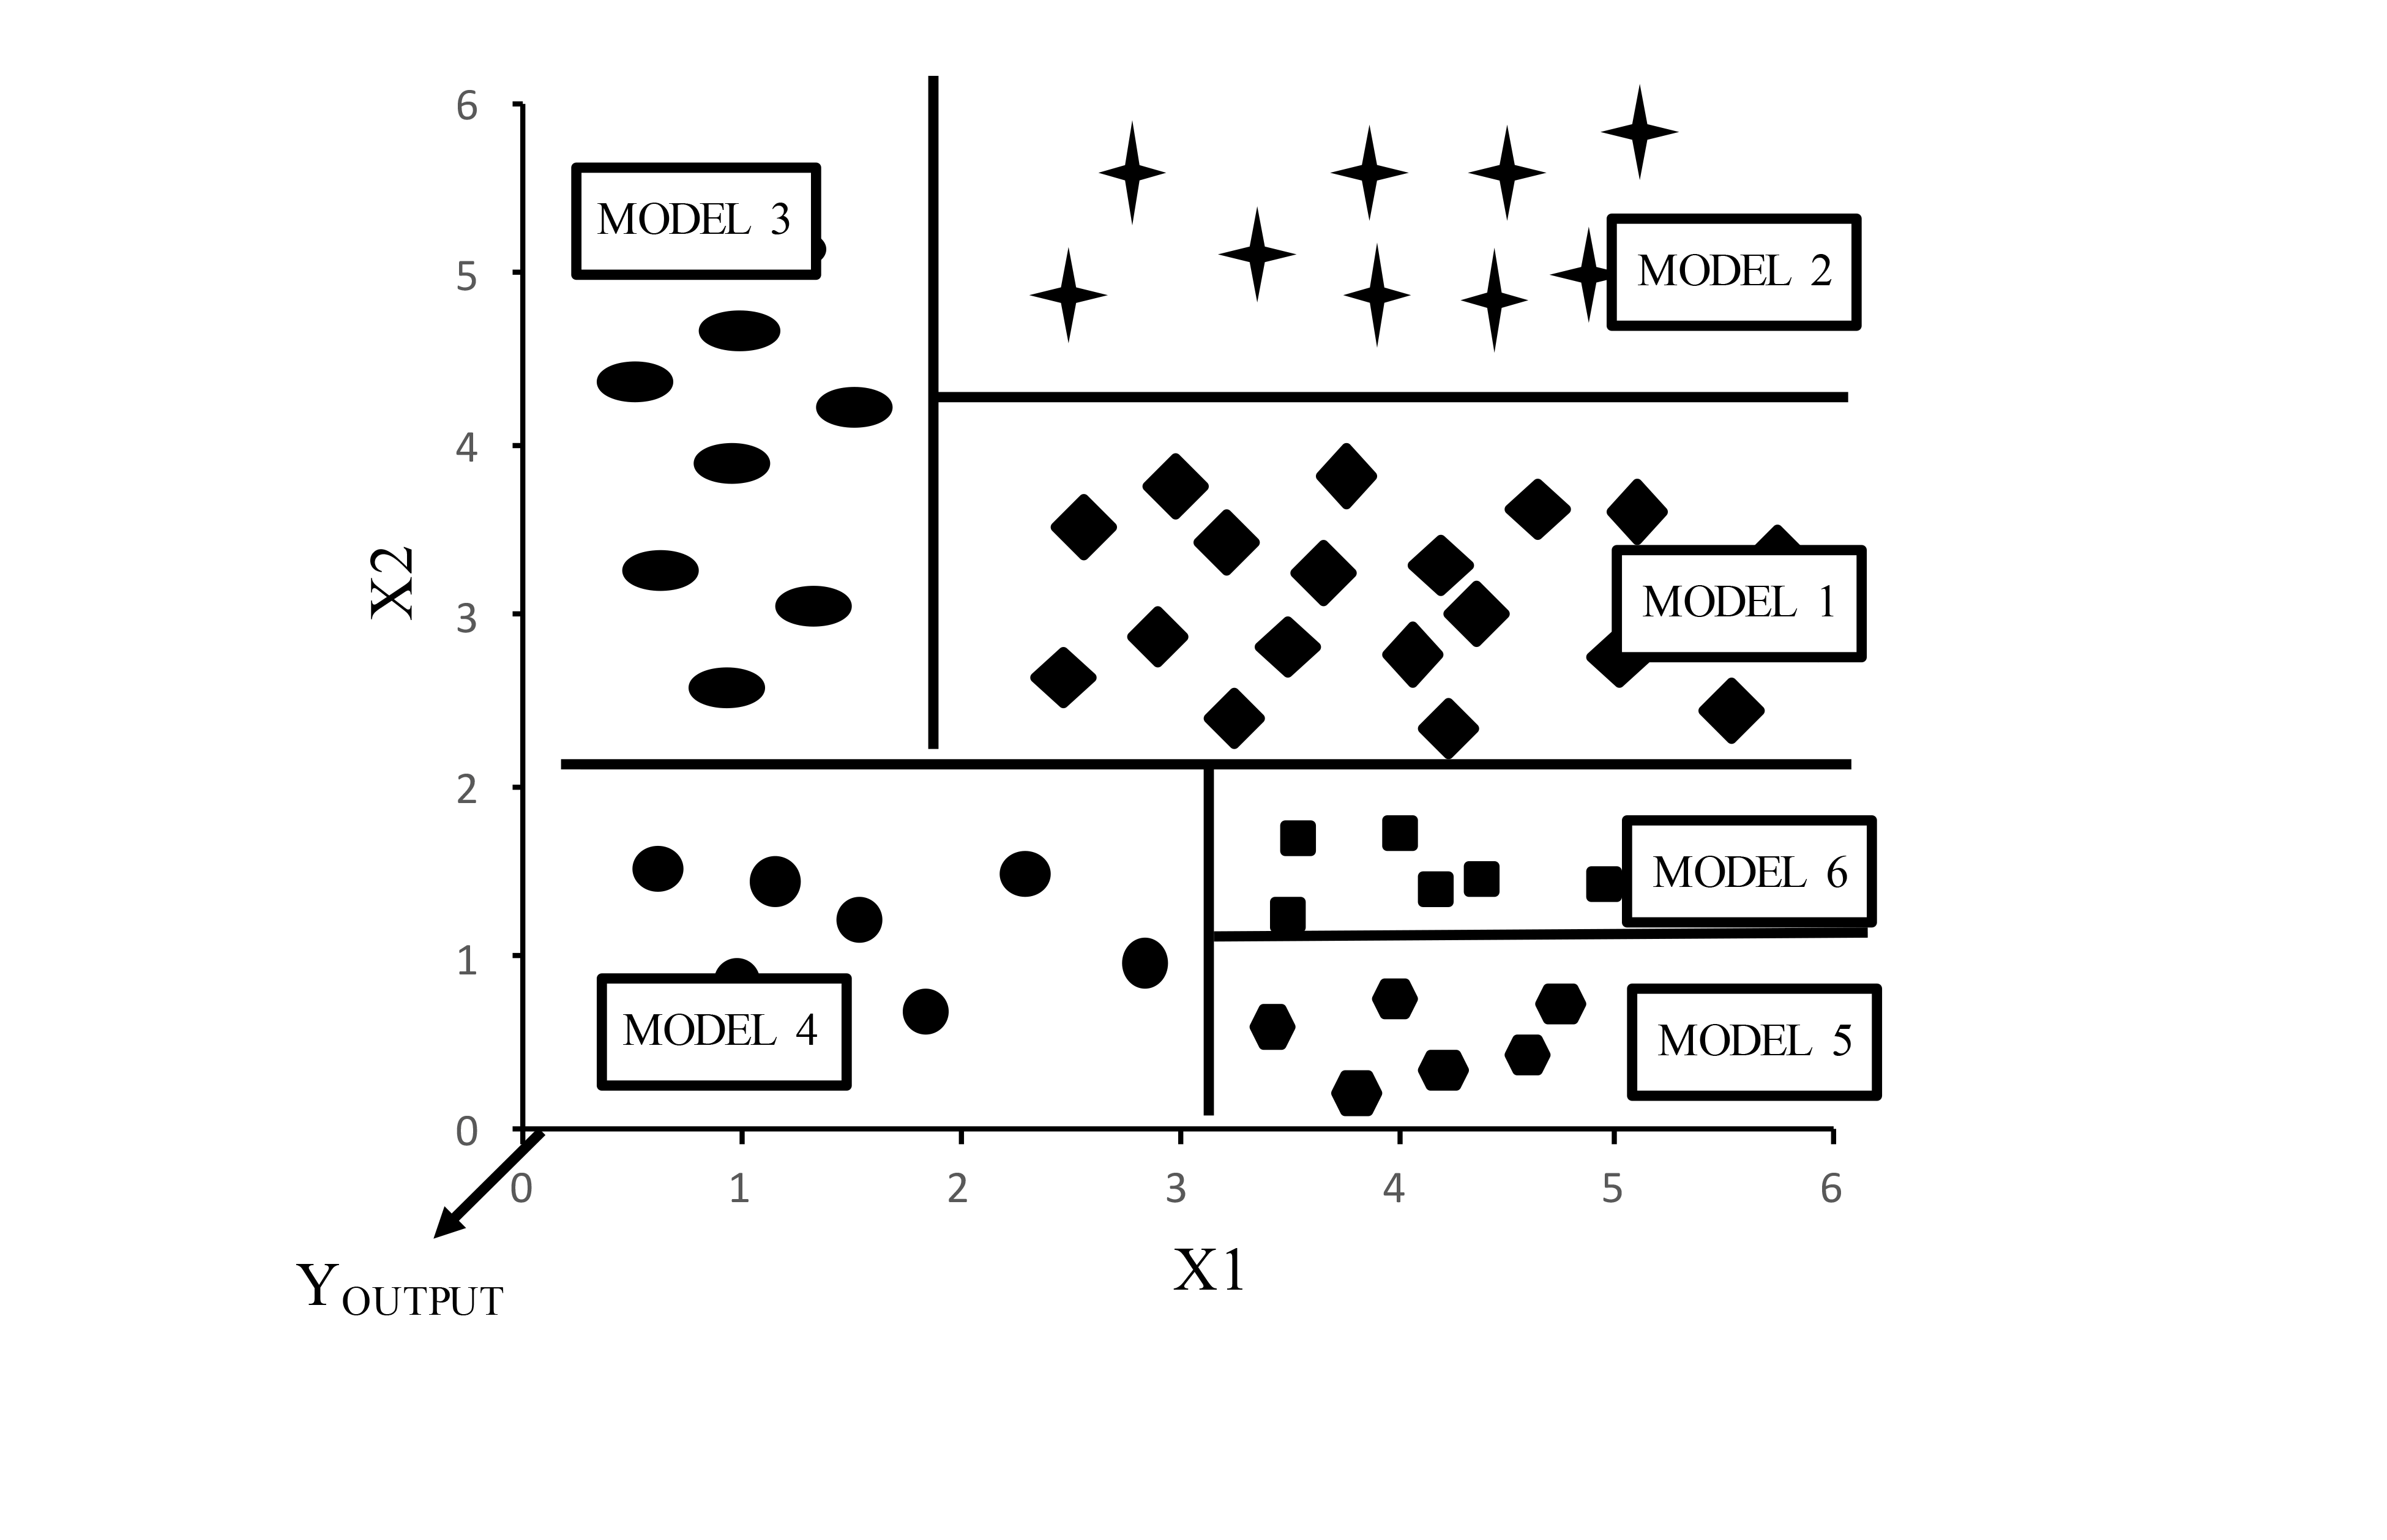
\includegraphics[height=7cm]{splits.png}
% \caption{Splitting of the input space (X1 x X2) by M5' model tree algorithm}
% \label{fig5}
% \end{figure}

% \section{Adding another section}
% You can show a lot of figures together like these Figures \ref{fig61}, \ref{fig62}, \ref{fig63} below.
% \begin{figure} [!htbp]
% \centering    
% \subfigure[Caption1]{\label{fig61}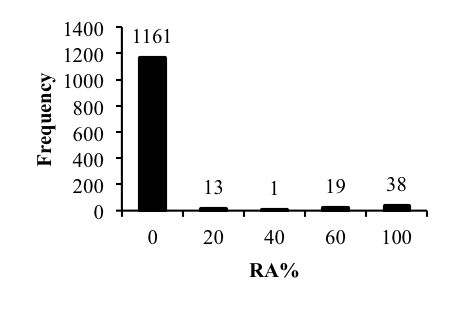
\includegraphics[width=42mm]{data1.png}}
% \subfigure[Caption2]{\label{fig62}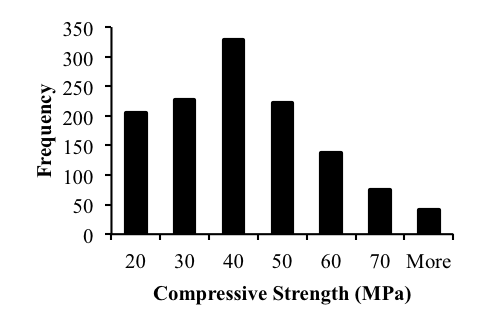
\includegraphics[width=42mm]{data2.png}}
% \subfigure[Caption3]{\label{fig63}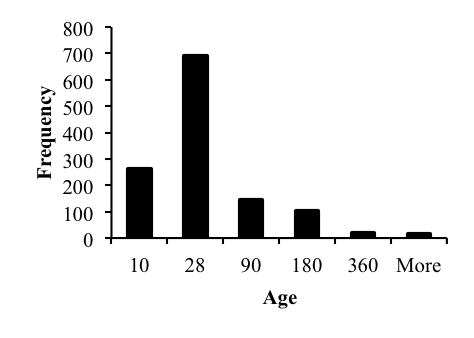
\includegraphics[width=42mm]{data3.png}}
% \caption{Figures sample}
% \end{figure}
% You can add lists into the text like this. 
% \begin{itemize}
% \settowidth{\leftmargin}{{\Large$\square$}}\advance\leftmargin\labelsep
% \itemsep3pt\relax
% \renewcommand\labelitemi{{\lower1pt\hbox{\small$\square$}}}
% \item	Some sample text item 1. 
% \item You may refer to tables \ref{tab1} 
% \item Or figures \ref{fig61}
% \end{itemize}

% Tables can be added like this
% \begin{table}[!htbp]
% \centering
% \caption{Sample table}
% \label{tab1}
% \begin{tabular}{llll}

% \hline
% Column 1 & Column 2 & Column 3       \\\hline
% 1         & Data1 & 13.41179 & 0.9492839 \\
% 2            & Data2 & 13.39824 & 0.9492952\\\hline
% \end{tabular}
% \end{table}



%% Discussion - Discuss the issues that you have got in the system, an idea about how you are trying to solve those. 
% Chapter Template

\chapter{Discussion} % Main chapter title

\label{Chapter 4} % Change X to a consecutive number; for referencing this chapter elsewhere, use \ref{ChapterX}

\lhead{Chapter 4. \emph{Discussion}} % Change X to a consecutive number; this is for the header on each page - perhaps a shortened title

\section{Properties of the system}

Here, we prove the safety and liveness properties of the system.

\subsection{Safety}

Since, we adding users in each round. Therefore, if we use a fixed maturity duration for a bond coin. Then in every round, we have some outgoing users and some incoming users.\\
Also, since the threshold for committing a block is two-thirds of the number of bond coins. Hence, between two consecutive rounds there will be atleast one honest user who has committed the block in that round. Since, the new bond coins are only allocated if the user's hashblock matches with the latest hash. Hence, if an honest user commits a block with bid $x$ and another honest user has committed a block with bid $y$ in the past when it had owned a bond coin, then $y$ must appear in the ledger of $x$.\\
Now, since more than two-thirds of the users are honest and more than two-thirds of the votes are needed for successful commit, hence a block would be committed only if atleast one-half of honest users commit it. And, honest users get consensus only if the block is correct hence the Safety property is guaranteed.

\subsection{Liveness}

Since, more than two-thirds of the users are honest, and a transaction can be accepted within k blocks, hence, it would be picked up by atleast one honest user and broadcasted to others. In case the highest priority block proposer is not an honest user, and the user sends two different sets of blocks then consensus would fail and a new consensus would take place with new priorities. If the highest priority block proposer sends out only one block and doesn't include this transaction then even though this block gets committed there is a high chance that an honest user will include it within k blocks. Hence, liveness property is guaranteed.

\section{Problems in System Design}

Here, we note some of the problems and boundary cases that might occur during the design and execution of the system and we try to give some plausible solutions.

\begin{enumerate}
    \item We know that CashCoins are liquid and can be transferred from one user to another. But, what if a user wants to transfer his voting rights to another user? If this user simply transfers it then he would also have to share the public-private key associated with this coin, but these are digital quantities and can be copied and can lead to the free-rider problem.\\
    Solution : Here, we assume that BondCoins are illiquid and non-transferable. If some user wants to transfer them, then he first has to convert the Coin to CashCoin and send these to the target user who then can convert these back to a BondCoin. This also avoids the free rider problem as when the target user gets his BondCoin, he would also get a new key pair associated with it.
    \item The bond coins are going to be minted using PoW. Once, all the bond coins are minted, the system adopts PoS system. PoW means we are finding some nonce which satisfies some properties, (In case of bitcoin, it had to be less than a given number). But, here the each bond coin is associated with a public and a private key pair which satisfy their own properties. How does the two gets associated?\\
    Solution : Here, the nonce and key-pairs are not related. A user can get a key pair even when PoS has taken over. We use El Gamal Cryptosystem for getting the private-public key pair associated with the BondCoin. This Cryptosystem is based on Elliptic Curve Cryptography (ECDLP) and provides better security with lesser key size. The Base point is common for all users. The private key can be decided by the winner of the current round randomly and based on it a public key can be chosen. But, once its decided, the user cannot change it and has to wait till the BondCoin matures. If he wants to change it then he would have to convert it to CashCoin and then again to BondCoin to choose a new one.
    \item What happens if a user who already owns a BondCoin wins another round while PoW consensus is active?\\
    Solution : If a user wins another round while PoW consensus is active, then he gets to commit that block but the BondCoin that is minted gets added to his account as CashCoin without any penalty. This is done to make sure that each validators has equal voting rights and hence own only one BondCoin with them.
    \item Here we note that PoW algorithm is only for minting bond coins. So, do the users don’t transact till all the bond coins are minted or does the peer minting the next bond coin becomes the leader for that round and commits the block of transactions to the ledger and once all the minting is over, PoS takes over and only those peers can take part in validation who are holding the bond coins?\\
    Solution : Here, we go with the choice that when the PoW consensus is active, the users can still transact and transaction fees are not taken from them. This is done to invite new users to the system and to increase the validators in the system. To incentivise users to participate in the consensus, the BondCoin minted in the current round is paid to the winner of the current round. Note that even after winning once, the users would still want to participate in the consensus to increase the CashCoins in their account.
    \item Each BondCoin comes with a maturity duration d. How is this maturity duration decided? What happens to the keys of the BondCoin once it gets expired and gets converted into CashCoin?\\
    Solution : Currently, this maturity duration is kept as a constant. Eg: 1 month. And, we plan to decide this value emphirically. Each BondCoin comes with a manufacture date, which is stored in the ledger. Once a BondCoin is expired, it gets added as CashCoins to the user account and the keys become useless. This process takes place the first time user transacts after his BondCoin is expired. If he tries to vote using the old keys then his vote is discarded during the expiration check phase.
    \item Since, the CashCoins are not converted automatically to BondCoins, what happens when there is no BondCoin left in the system?\\
    The situation where no BondCoins are left in the system is hard to occur. As the BondCoins in the system decrease, the transaction fees would decrease. In this case, automatically the demand for BondCoins would increase as the few users who are owners of the last few BondCoin would enjoy more shares of the transaction fees by themselves. But, no BondCoin situation can occur only when the last of BondCoins also got matured automatically and no other user converted their CashCoin into a BondCoin before their expiration which would bring the system to a standstill. If there are no BondCoin in the system then there would be no validators in the system and no user would be able to transact and hence the CashCoins in their account would become useless. In this unlikely situation, we suggest that the PoW system is restarted so that the BondCoins in the system can be increased and users can enjoy transactions without paying the fees and do not have to leave the system.
    \item Why is there a penalty for converting BondCoin to CashCoin? How is its amount fixed?\\
    Solution : The BondCoin is like a contract given to user to participate in the validation process during its maturity period. Its like a fixed deposit done in bank, on which you get the interest during the period but you can use the money only after it matures, if you take the money out before it matures then you have to pay a penalty. In a similar way, this penalty is imposed on those users who want to do away with their responsibility of participating in the validation process. The amount is fixed based on the number of BondCoins currently in the system. More the number of BondCoins, more the penalty.

\end{enumerate}

\section{Plausible attacks}

Here, we assume that the block has been prepared and validators are decided, we only need to consider attacks that can be made while committing this block to the ledger.

\begin{enumerate}
    \item Adversary can be the owner of majority of bond coins. Adversary can make multiple accounts with only enough cash coin to convert them into bond coins.
    \item If in response to above, the bond coins are made larger in number then network attacks would be easier. Adversary may be able to slow down the network or partition some nodes.
    \item Instead of buying the bond coins itself, adversary may hack prominent accounts holding bond coins. It's useful as they are gonna be valid for duration d.
\end{enumerate} 
%% Discussion - Discuss the issues that you have got in the system, an idea about how you are trying to solve those. 
% Chapter Template

\chapter{Distributed Algorithm} % Main chapter title

\label{Chapter 5} % Change X to a consecutive number; for referencing this chapter elsewhere, use \ref{ChapterX}

\lhead{Chapter 5. \emph{Distributed Algorithm}} % Change X to a consecutive number; this is for the header on each page - perhaps a shortened title

\section{Assumptions}

We take the following assumptions for our distributed system :

{
\singlespacing
\begin{itemize}
    \item Each user has a unique id
    \item Each user knows other users
    \item Each user is a node in itself
    \item More than 2/3rd of the users (or specifically the committee members) are honest (non-faulty and form the largest sub) in the system (non-faulty)
    \item New requests for bond coin keep coming in
    \item Each user has a unique public address known to other user while its active
    \item Asynchronous system (Network Faults can happen)
    \item Eventually synchronous system (Eventually all network faults would be resolved)
    \item Reliable connection
    \item Each function is executed atomically
\end{itemize}
}

\section{Abbreviations}

Following are the abbreviations used to denote some fields and classes :
{
\singlespacing
\begin{itemize}
    \item id = User's ID
	\item mt = Transaction Type
	\item sid = Sender's ID
	\item rid = Reciever's ID
	\item t = Timestamp, can also be the id of the last block seen by the user to avoid time conflicts
	\item cc = CashCoin
	\item bc = BondCoin
	\item pk = Public Key of a user
	\item sk = Secret Key / Private Key of a user
	\item val = Transaction amount value that a user wants to send to another user
	\item h = hash obtained on applying a verifiable random function on the message using sk
	\item p = proof for verifying the hash of a message using that user's pk
	\item pa = public address for committee to communicate with this node during consensus
	\item fb = First Block in which a user starts giving consensus
	\item lb = Last Block after which a user stops giving consensus
	\item cps = Cryptocurrency Participation Score
	\item k = The number of blocks till which a transaction is valid. If a transaction is more than 
\end{itemize}
}

\section{Message Types}

Following messages will be exchanged in the system :

{
\singlespacing
\begin{enumerate}
    \item Transfer : Message gossiped by the a node with id sid to send val amount of cashcoins to a node with id rid at timestamp t.
    \begin{verbatim}
Message Transfer
{
    mt
    sid
    rid
    val
    tc
    t
    h
    p
}
    \end{verbatim}
    \item RequestBC : Message requesting to convert cashcoin to bondcoin and become a member of the committee.
    \begin{verbatim}
Message RequestBC
{
    mt
    sid
    pa
    tc
    t
    h
    p
}
    \end{verbatim}
    \item RequestCC : Message requesting to convert bondcoin to cashcoin before maturity.
    \begin{verbatim}
Message RequestCC
{
    mt
    sid
    tc
    t
    h
    p
}
    \end{verbatim}
    \item ChangePK : Message requesting to change pk.
    \begin{verbatim}
Message ChangePK
{
    mt
    sid
    pk // New Public Key
    tc
    t
    h
    p
}
    \end{verbatim}
    \item Join : Message requesting to join the system as a new user. The new id would be mentioned in the next few blocks as confirmation.
    \begin{verbatim}
Message Join
{
    mt
    pk
    tc
    t
    h
    p
}
    \end{verbatim}
    \item BlockCommit : Message broadcasted to give info about a new block.
    \begin{verbatim}
Message BlockCommit
{
    mt  // type of message
    sid // sender id
    block // block list element
    h // hash
    p // proof
}
    \end{verbatim}
\end{enumerate}
}

\section{Variables stored at each node}

{
\singlespacing
\begin{enumerate}
    \item myid = The ID of the user. This is allocated by the system when the user joins for the first time. It is an unsigned number and 0 is reserved for nodes who haven't joined yet. This id is used to index a user's information in the database.
	\item mysk = Private/Secret Key of the user. This is the only private state of the node (same as in algorand) and is used to sign the messages sent by it.
	\item mypk = The public key of the user. This key is advertised by the node so that other nodes can use it to verify its messages, it is unique to a node.
	\item mypa = The public address of the user for other users to send message when it takes part in the consensus. This address is only required when the user requests for a BondCoin.
	\item myfb = The most recent block from which user start participating in consensus
	\item mylb = The most recent block after which user stop participating in consensus
	\item mytc = User's transaction count to distinguish between two of its transaction in the same block, alternative to timestamp.
	\item hblock = Hash of the newest block seen.
	\item nusr = Number of users in the system, used to give id to a new user.
	\item bcuncommitted = Blocks heard but not yet committed. It is a priority queue arranged with respect to bid.
	\item trnuncommitted = Transactions heard but not committed. Transactions are arranged according to last block seen t and no duplicates are stored. The transactions are only stored by prospective BondCoin owners.
	\item nbr = Nearest neighbours in the network, information given by the network. This information is used for Distributed Broadcast of messages.
	\item bcq = A queue of users who have the bond coins and are participating in the consensus or going to participate in the future. No user can be twice in this q at a time. users in the queue can be accessed using their ids. Its like a dictionary but like a priority queue arranged using lb or fb. Implemented using double ended queue.
    Each element of the queue has following definition.
\begin{verbatim}
QueueElement BCUser
{
    id // ID of the user
    pk // Public Key of the user
    pa // Public Address of the user
    fb // first Block giving consensus
    lb // last Block giving consensus
    active // 1 if user is participating in consensus
}
\end{verbatim}
    \item usrd = A dictionary of users which maps a user's id (key here) to all the information about that user.
The values in the dictionary would have following definition
\begin{verbatim}
DictionaryKey id
DictionaryValue User
{
    pk
    lastpa
    cc
    cps
    fb  // the first block from which it joined
}
\end{verbatim}
    \item bcl = A list of blocks which acts as a unified ledger. Each block is a collection of transactions. Each transaction contains the original request and the response given after the consensus. A transaction is included in a block only if it is successful.
Each transaction has the following definition.
\begin{verbatim}
ListElement Transaction
{
    treq // Transaction Request, JSON string
    tres // Transaction Response, JSON string
}
\end{verbatim}
Each transaction can be of following types :
    \begin{enumerate}
        \item Transfer
        \begin{verbatim}
treq = 
{
    mt = `Transfer'
    sid
    rid
    val
    tc
    t
    h
    p
}
tres = 
{
    valfinal // Value transferred to the reciever after 
deducting the transaction fees
}
        \end{verbatim}
        \item RequestBC
        \begin{verbatim}
treq = 
{
    mt = `RequestBC'
    sid
    pa
    tc
    t
    h
    p
}
tres = 
{
    fb
    lb
}
        \end{verbatim}
        \item RequestCC
        \begin{verbatim}
treq = 
{
    mt = `RequestCC'
    sid
    tc
    t
    h
    p
}
tres =
{
    lb
    valfinal // Value to be added to user's account after 
putting fine on it. Fine put on the user as transaction 
fees for converting bc to cc before maturity.
}    
        \end{verbatim}
        \item ChangePK
        \begin{verbatim}
treq = 
{
    mt = `ChangePK'
    sid
    pk // New Public Key
    tc
    t
    h
    p
}
tres =
{
    fb // ID of the block from which the new public key 
would be valid
}    
        \end{verbatim}
        \item Join
        \begin{verbatim}
treq = 
{
    mt = `Join'
    pk
    tc
    t
    h
    p
}
tres =
{
    id // id of the new user
    fb // ID of the block from which the user would be valid
}
        \end{verbatim}
    \end{enumerate}
Each block has the following definition.
\begin{verbatim}
ListElement block
{
    bid // BlockID
    bpid // BlockProposerID
    tlist // List of Transaction Objects
    memlist // List of ids of BondCoin holders who participated 
in this round
    trnfees // Fees earned by each BondCoin owner in this round
    retirelist // List of ids of BondCoin holders who retire 
after this round
    joinlist // List of ids who are given allocated new bondcoins
    nusr // No. of users in the system after accepting new join 
requests in this block
    hprev // hash of previous block
    hq // hash of bcq after applying changes of this block of 
transactions
}    
\end{verbatim}
\end{enumerate}
}

\section{Initialisation}
{
\singlespacing
\begin{enumerate}
    \item myid = 0 or id given by the system when joined the first time
	\item mysk = secret key chosen by me
	\item mypk = public key corresponding to mysk
	\item mypa = public address given by the network to which other users can send messages to communicate with me
	\item mytc = 0 or transaction count of the last transaction
	\item hblock = 0 or hash of the last block in bcl
	\item nusr = 0 or nusr in the last block in bcl
	\item bcq = empty or Queue of users mirrored from a bondcoin holder
	\item usrd = empty or Dictionary of users mirrored from a bondcoin holder
	\item bcl = empty or List of blocks mirrored from a bondcoin holder
	\item bcuncommitted = empty
	\item trnuncommitted = empty
	\item nbr = nearest neighbours in the network, information given by the network
\end{enumerate}
}

\section{Functions}

\subsection{Abstract Functions}
These functions are called by other functions and serve specific tasks.
\begin{enumerate}
    \item Prepare : This function is called before pushing or broadcasting any message. This function sets t, h, p in a message
    \begin{lstlisting}
Abstract Prepare (Message M)
{
    if M.mt in {Transfer, RequestBC, RequestCC, ChangePK, Join} :
        // Can use some mutex while assigning timestamp to avoid 2 transactions getting same timestamp. Instead using tc (transaction count) here. Use mutex while assigning the tc value and incrementing it.
        mytc++
        M.tc = mytc
        M.t = bcl[-1].bid
    M.h = M.p = 0
    (M.h, M.p) = VRF (M, mysk)
}
    \end{lstlisting}
    \item Push : This function sends the message to all the bcowners in the user's queue. Put flag as 1 to send to only active members and 2 to send to all members.
    \begin{lstlisting}
Abstract Push (Message M, flag)
{
    for usr in bcq :
        if flag == 1 and usr.active == 0 :
            break
        if usr.active == -1 :
            continue
        Send M to usr.pa
}
    \end{lstlisting}
    \item Broadcast : This function is used to broadcast a message to the network.
    \begin{lstlisting}
Abstract Broadcast (Message M)
{
    // Implementing distributed broadcast here
    for usr in nbr :
        Send M to usr
}
    \end{lstlisting}
    \item Same : This function is for comparing two messages
    \begin{lstlisting}
Abstract same (treq t1, treq t2)
{
    // Here, we can compare sid but its not generic for all kinds of messages and following four will be enough
    // Added timestamp to distinguish between 2 similar transactions sent in the same block

    // Compare transaction type
    if t1.mt != t2.mt :
        return false
    
    // Compare transaction count
    if t1.tc != t2.tc :
        return false

    // Compare block of transaction
    if t1.t != t2.t :
        return false
    
    // Compare hash
    if t1.h != t2.h :
        return false
    
    // Compare proof
    if t1.p != t2.p :
        return false

    // This means that it is the same transaction, return true
    return true
}
    \end{lstlisting}
    \item Response : This function returns if the transaction was successful.
    \begin{lstlisting}
Abstract Response (Message M)
{
    // Check till k blocks if the transaction has been committed
    for i = M.t + 1 to M.t + k :
        // Check in every TCommit time if the new block has been added to bcl, here TCommit is avg commit time of a block
        while bcl[-1].bid < i :
            wait(TCommit)
        
        // Check in every transaction of the block to find own transaction
        for trn in enumerate(bcl[i].tlist) :
            if same(trn.treq, M) :
                return (true, trn.tres)
    
    // No match means the transaction wasn't accepted
    return (false, null)
}
    \end{lstlisting}
    \item : validUser : This function checks if the user has joined the system ie. it is a valid user or not.
    \begin{lstlisting}
Abstract validUser()
{
    // Check if the user is joined or not
    if myid == -1 :
        raiseError (' User not yet joined in the system ')
}
    \end{lstlisting}
    \item checkBCOwner : This function checks if a usr is BCOwner, pass flag as 1 to search only in current members and flag as 2 to search in all users.
    \begin{lstlisting}
Abstract checkBCOwner(id, flag)
{
    for usr in bcq :
        if flag == 1 and usr.active == 0 :
            break
        if usr.active == -1 :
            continue
        if usr.id == id :
            return true
    return false
}
    \end{lstlisting}
    \item verify : This function verifies a message sent by a user.
    \begin{lstlisting}
Abstract verify(Message M)
{
    if M.mt == Join :
        return VRFVerify(M, M.pk, M.h, M.p) // VRFVerify takes care of hashing when M.h = M.p = 0
    return VRFVerify()
}
    \end{lstlisting}
    \item ExecuteBlock : This function executes the transaction of a new block. If flag is 0 means just verifying the block, if flag is 1 means executing it.
    \begin{lstlisting}
Abstract ExecuteBlock (block, bcq, usrd, flag)
{
    if flag == 0 :

        if block.bid != bcl[-1].bid + 1 :
            return false
        
        // Can also check for bpid and put a hash, proof accordingly here

        // Can also check for priority of block proposer

        // Can make the above two commented checks in the function collecting block proposals itself
        
        // Check if previous hash matches
        if hblock != block.hprev :
            return false

        <Check if memlist matches the current active users in bcq>

        bcq = copy(bcq)
        usrd = copy(usrd)
        input = output = 0
        // Can also check the different memberlist or remove them entirely except memlist

    // Remember to execute RequestCC after RequestBC, can give a pass thru tlist at the end for RequestCC
    for trn in block.tlist :
        if flag == 0 and verify(trn.treq) == false :
            return false
        switch(trn.treq.mt)
            case Transfer :
                usrd[trn.treq.sid].cc -= val
                usrd[trn.treq.rid].cc += trn.tres.valfinal
                if flag == 0 :
                    if usrd[trn.treq.sid].cc < 0 :
                        return false
                    input += val
                    output += trn.tres.valfinal
            
            case RequestBC :
                usrd[trn.treq.sid].cc -= 1
                bcu = newBCUser
                bcu.id = trn.treq.sid
                bcu.pk = usrd[bcu.id].pk
                bcu.pa = trn.treq.pa
                bcu.fb = trn.tres.fb
                bcu.lb = trn.tres.lb
                bcu.active = 0
                bcq.push(bcu)
                if flag == 0 :
                    if usrd[trn.treq.sid].cc < 0 :
                        return false
                    input += 1
                    output += 1
            
            case RequestCC :
                bcq[trn.treq.sid].active = -1
                usrd[trn.treq.sid].cc += trn.tres.valfinal
                if flag == 0 :
                    input += 1
                    output += trn.tres.valfinal
            
            case ChangePK :
                usrd[trn.treq.sid].pk = trn.treq.pk
            
            case Join :
                usrd[trn.tres.id] = new User
                usrd[trn.tres.id].pk = trn.treq.pk
                usrd[trn.tres.id].lastpa = 0
                usrd[trn.tres.id].cc = 0
                usrd[trn.tres.id].cps = thres // here thres is the threshold
                usrd[trn.tres.id].fb = trn.tres.fb
    
    if flag == 0 :
        output += len(memlist)*block.trnfees
        if input != output :
            return false
        
        if len(usrd.keys) != block.nusr :
            return false

    // Add fees to members account
    for id in memlist :
        usrd[id].cc += block.trnfees
    
    // Pop retired members from bcq
    while bcq != empty and bcq.head.lb == bcl[-1].bid :
        bcq.pop()
    
    if flag == 0 :
        hq = hash(bcq)
        if hq != block.hq :
            return false
        return true
    
    // Means flag = 1
    hblock = hash(block)
    nusr = block.nusr
    
}
    \end{lstlisting}
\end{enumerate}

\subsection{Threads}
These functions run independently and may not be atomic.
\begin{enumerate}
    \item Sentinel : This thread runs at the start and tries to get user updated with the latest blocks.
\begin{lstlisting}
Thread Sentinel ()
{
    // run at all times except stops only when user goes offline

    time.reset()
    while(true) :
        
        // Resync if its past resynchronisation period
        if time.gone() > tresync :
            < Explicitly get missing blocks from other users and put it in bcuncommitted and broadcast them too >
            time.reset()

        
        // Commit the uncommitted block if any
        while bcuncommitted != empty and bcuncommitted.head.bid == bcl[-1].bid + 1 : // Here, in case of a bcl empty would need to add another condition, instead either put a dummy block at the start of bcl with id 0 or replace bcl[-1].bid with len(bid), if going with the former can also get the genesis block as a response to the Join message.
            bcl.append(bcuncommitted.head)
            bcuncommitted.pop()
            ExecuteBlock(bcl[-1], bcq, usrd, 1)
        
        // Listen for new message
        M = Listen() 

        // Verify only if not a new user
        if bcl != empty :
            verify(M)

        // Commit Message
        if M.mt == BlockCommit :
            
            // Already updated
            if bcl[-1].bid >= M.block.bid :
                continue
            else :
                bcuncommitted.push(M.block)

                // Only broadcast further if in the network
                if myid != 0 :
                    M.sid = myid
                    Prepare(M)
                    Broadcast(M)

        else if M.mt in {Transfer, RequestBC, RequestCC, ChangePK, Join} :
            // If I am a member
            if bcl[-1].id < mylb :
                trnuncommitted.push(M) // push removes duplicates and puts in the correct position in the queue, it also removes a transaction if already committed using function Response, and removes those which are already expired

            // If I am not an active member ignore
            else :
                continue

                
}
\end{lstlisting}
    \item Participate : This thread runs for the time the user has to participate in the consensus.
\begin{lstlisting}
Thread Participate()
{
    // mylb takes care that I am a member, for voting will also check if an active member, in normal operation the thread itself will destroy
    while bcl[-1].bid < mylb :
        <remove transactions from truncommitted who are accepted and those for which this block is the last hope and still they are not valid>
        
        // Take part only if in next block we are an active bcowner
        if bcl[-1].bid + 1 >= myfb :
            if <Proof of stake/current block makes me a proposer> :
                <Validate the transactions seen so far>
                <Propose a block>
                <Put priority>
                <Push it to the current active members>
                <Add it to own proposal list>
            
            while <proposal time> :
                <pop a new proposal>
                <check the validity of proposal>
                <put it as this round's block if highest priority> 

            <vote for the highest proposal seen>

            while <voting time> :
                <pop a vote>
                <add the vote>
                <see if the votes for a particular block exceeds 2/3rds of the total votes>
                <if it does commit this block and broadcast>
                <break> 

        <wait till new block is committed>
        <if not committed within some time restart consensus>

    destroy truncommitted
    Stop this thread
}
\end{lstlisting}
\end{enumerate}

\subsection{Public Functions}
These functions can be called directly by the user or are called depending on the events triggered by actions of the user.
\begin{enumerate}
    \item Wakeup : This function is called when the node boots up.
    \begin{lstlisting}
Wakeup () :
    Start thread Sentinel()
    \end{lstlisting}
    \item Shutdown : This function is called when the node is shutting down.
    \begin{lstlisting}
Shutdown () :
    If myid in bcq :
        <Push RequestCC>
        <Wait till the request is accepted>
    Stop thread Sentinel()
    \end{lstlisting}
    \item Transfer : This function is called by the user when it wants to transfer money to another user.
    \begin{lstlisting}
Transfer (rid, val)
{
    // Check if the user is joined or not
    validUser()
    
    // Check if reciever is valid or not
    if rid > nusr :
        raiseError (' Reciever is not valid ')

    // Check if val is valid
    if val > usrd[myid].cc :
        raiseError (' Not enough cashcoins to send ')

    // Prepare the message for sending
    mtransfer = new Message
    mtransfer.mt = Transfer
    mtransfer.sid = myid
    mtransfer.rid = rid
    mtransfer.val = val

    // Set tc, t, h, p
    Prepare (mtransfer)

    // Send the message to all the bcowners including those who have not yet started
    Push (mtransfer, 2)

    // Get response for the transaction
    (success, tres) = Response (mtransfer)

    // As the user's own accounts will also be handled in a general way, no use of tres here

    // return if the transaction was successful
    return success
}
    \end{lstlisting}
    \item RequestBC : This function is called by the user when it wants to participate in the consensus
    \begin{lstlisting}
RequestBC ()
{
    // Check if the user is joined or not
    validUser()

    // Check if the user has enough cashcoins
    if 1 > usrd[myid].cc :
        raiseError (' Not enough cashcoins to convert to bondcoin ')

    // Prepare the message for sending
    mrequestBC = new Message
    mrequestBC.mt = RequestBC
    mrequestBC.sid = myid
    mrequestBC.pa = mypa

    // Set tc, t, h, p
    Prepare (mrequestBC)

    // Send the message to all the bcowners including those who have not yet started
    Push (mrequestBC, 2)

    // Get response for the transaction
    (success, tres) = Response (mrequestBC)

    if success :
        // Set myfb and mylb
        myfb = tres.fb
        mylb = tres.lb
        create tnuncommitted
        start thread Particpate()

    // return if the transaction was successful
    return success
}
    \end{lstlisting}
    \item RequestCC : This function is called by the user when it wants to convert its bondcoin before maturity.
    \begin{lstlisting}
RequestCC ()
{
    // Check if the user is joined or not
    validUser()

    // Check if the user is in bcq
    if not checkBCOwner(myid, 2) :
        raiseError (' User not in BCOwner queue ')

    // Check if the user holds bc now
    if (bcl[-1].bid+1) == lb :
        raiseError (' User in BCOwner queue but this is last block ')
    
    // Prepare the message for sending
    mrequestCC = new Message
    mrequestCC.mt = RequestCC
    mrequestCC.sid = myid
    
    // Set tc, t, h, p
    Prepare (mrequestCC)

    // Send the message to all the bcowners including those who have not yet started
    Push (mrequestCC, 2)

    // Get response for the transaction
    (success, tres) = Response (mrequestCC)

    if success :
        // Set mylb
        //myfb = tres.fb
        mylb = tres.lb
        destroy trnuncommitted // can also just clear it
        Stop Thread Participate()

    // return if the transaction was successful
    return success
}
    \end{lstlisting}
    \item ChangePK : This function is called by the user when it wants to update its public key.
    \begin{lstlisting}
ChangePK (newpk)
{
    // Check if the user is joined or not
    validUser()

    // Prepare the message for sending
    mchangePK = new Message
    mchangePK.mt = ChangePK
    mchangePK.sid = myid
    
    // Set tc, t, h, p
    Prepare (mchangePK)

    // Send the message to all the bcowners including those who have not yet started
    Push (mchangePK, 2)

    // Get response for the transaction
    (success, tres) = Response (mchangePK)

    if success :
        // Set mypk
        mypk = newpk

    // return if the transaction was successful
    return success
}
    \end{lstlisting}
    \item Join : Called by a user to join the system for the first time. The bcowners check if the public key provided by the user is unique or not. If it is the user is given a unique id after which the user can start using the system. On success, the user would start mirroring the previous blocks, queue of users and dictionary of users from any member of the system.
    \begin{lstlisting}
Join ()
{
    // Can check if the user already exists but it might happen that same client wants to join as multiple user so we allow it here.

    // Prepare the message for sending
    mjoin = new Message
    mjoin.mt = Join
    mjoin.pk = mypk
    
    // Set tc, t, h, p
    Prepare (mchangePK)

    // Send the message to all the bcowners including those who have not yet started
    Push (mjoin, 2)

    // Get response for the transaction
    (success, tres) = Response (mchangePK)

    if success :
        // Set myid
        myid = tres.id

    // return if the transaction was successful
    return success
}
    \end{lstlisting} 
\end{enumerate} 
%% Conçlusion and Future Works. 
% Chapter Template

\chapter{Conclusion and Future Works} % Main chapter title

\label{Chapter 6} % Change X to a consecutive number; for referencing this chapter elsewhere, use \ref{ChapterX}

\lhead{Chapter 6. \emph{Conclusion and Future Works}} % Change X to a consecutive number; this is for the header on each page - perhaps a shortened title

In this report, we saw how the number of validators for a POS system can be dynamic and may be determined by the market parameters. The POS systems were better than POW systems because they don't waste computational power in redundant tasks but POS systems itself has some drawbacks. The proposed system tries to solve some of these drawbacks. The crux of the proposed system lies in the fact that all the validators are given equal voting rights so that adversary is also ripped off of the probabilistic advantage of gaining the control of the system which is prevalent in the recently proposed systems such as Algorand. In this system, gaining half the currency of the system is not enough for the adversary. He must have control over more than half of the BondCoins i.e. more than half of the computation power. And, as these BondCoins come with an expiry, the task of the adversary becomes more difficult.

In future we would like to achieve the following objectives :
\begin{enumerate}
    \item We would like to explore how the system is affected if the maturity duration of a BondCoin is variable
    \item We would like to devise a method to ensure that a minimum number of validators are always there in the network at a given point of time
    \item We would like to explore how the system is affected if the BondCoin is also quantized. For eg : a group of users can combine their CashCoins to get one BondCoin. What would be the final vote of such a group of users?
    \item Till now, we have assumed that all the validators remain active all the time. We would like to explore what happens if some of the validators crash or go offline.
    \item We would like to tackle the geographical scalability of POS protocols and devise a solution for it.
    \item We would like to scale the implemented system and run benchmark tests on it.
    \item We would like to explore how charging fees for conversion of CashCoin to BondCoin affects the economy of the system.
    \item We would like to prove the system's correctness under weaker assumptions.
    \item Change the relation between BondCoins and transaction fees and analyse the new system.
\end{enumerate} 
%% Conçlusion and Future Works. 
% Chapter Template

\chapter{Related Works} % Main chapter title

\label{Chapter 7} % Change X to a consecutive number; for referencing this chapter elsewhere, use \ref{ChapterX}

\lhead{Chapter 7. \emph{Related Works}} % Change X to a consecutive number; this is for the header on each page - perhaps a shortened title

In this section, we see what other kinds of protocols have been proposed to solve the age old state machine replication problem.

\section{Bitcoin}

The protocol on which the cryptocurrency Bitcoin is transacted, this was the earliest of the blockchain protocols. It follows a Proof of work consensus wherein nodes compete among themselves to solve a hard problem. And, whoever solves the problem gets to mine the next block and is accordingly rewarded. The protocol is permissionless that is any user can join and completely decentralized as there is no central authority validating the transactions.

% \begin{itemize}
%     \item It’s a public blockchain, i.e. permission-less, where anyone can join.
%     \item The underlying technology components are cryptographic hash function, digital signature, private-and-public key encryption, peer-to-peer (P2P) network, and proof of work (POW) consensus algorithm.
%     \item The protocol allows users to conduct non-reversible transactions without having to explicitly trust a third-party.
%     \item Every node has the complete information on the blockchain, making the network a decentralized one.
%     \item Transactions contain unique transaction ID, input Bitcoin address, the number of Bitcoins to be transferred, and the output Bitcoin address of the recipient.
%     \item The transaction making process involves the initiator of the transaction, and ‘miner’, i.e. combination of special-purpose software, powerful hardware, and their user. The transaction initiator pays transaction fees to the miner, who tries to include the transaction in the next block. A block is processed in every 10 minutes, and the transactions included in that are then recorded in the blockchain. Creating a new block requires not only the transaction information of the current transaction, but also a reference to the last recorded block. The last recorded block isn’t known, and the miner needs to solve a complex cryptographic puzzle to find it, and this essentially involves a large number-crunching operation done at high-speed. For this, the miner needs to try one number after another, which requires high computing power. Majority of the participating nodes must approve the transaction. Since this is a decentralized network, it isn’t possible for anyone to capture majority of the computing power on the network, thus making the network very secure. Thus, while POW mining ensures high security of blockchain, it’s also computing-power-intensive, and requires high amount of energy.
%     \item The transaction making process involves the initiator of the transaction, and ‘miner’, i.e. combination of special-purpose software, powerful hardware, and their user. The transaction initiator pays transaction fees to the miner, who tries to include the transaction in the next block. A block is processed in every 10 minutes, and the transactions included in that are then recorded in the blockchain. Creating a new block requires not only the transaction information of the current transaction, but also a reference to the last recorded block. The last recorded block isn’t known, and the miner needs to solve a complex cryptographic puzzle to find it, and this essentially involves a large number-crunching operation done at high-speed. For this, the miner needs to try one number after another, which requires high computing power. Majority of the participating nodes must approve the transaction. Since this is a decentralized network, it isn’t possible for anyone to capture majority of the computing power on the network, thus making the network very secure. Thus, while POW mining ensures high security of blockchain, it’s also computing-power-intensive, and requires high amount of energy.
%     \item While the consensus mechanism requiring majority approval rules out foul play, it also creates scalability issues, since every node must load entire information on blockchain and participate in the transaction validation process. Bitcoin blockchain has recently implemented ‘Segregated Witness’ (SegWit) technology, which bypasses the limitation on block size, and separates signature information from the transaction data, to improve scalability of the network.
% \end{itemize}

\section{Ethereum}

Ethereum blockchain has many similarities with Bitcoin protocol, for e.g.: It’s a public, permission-less blockchain; It uses the same technological backbones, for e.g. cryptographic hash function, private-and-public key encryption, P2P network, etc; POW consensus algorithm is used; There’s a native cryptocurrency, called Ether. Ether has the second highest market cap, behind only Bitcoin.

However, unlike Bitcoin, which was built for allowing crypto payment transactions over a decentralized network, Ethereum was designed with much larger objectives in mind. Ethereum provides a blockchain platform, using which developers can launch their own blockchain projects, including their own cryptocurrencies. The platform, commonly called as ‘Ethereum Virtual Machine’ (EVM), has been used to launch over 1,000 DApps. Famous cryptocurrency projects such as VeChain and OmiseGo have been launched using EVM.\\
Smart contracts make this possible. Smart contracts are pieces of code, which allows execution of legal functions, for e.g. taking control of an entity based on certain conditions, and transferring crypto tokens based on fulfilling required conditions. Smart contracts on the Ethereum platform are codes using Ethereum’s proprietary language Solidity, which is inspired by C++, Java, Python and JavaScript.\\
DApps are applications where the backend code runs on a decentralized blockchain, and comprises of smart contracts. Ethereum has made wider adoption of blockchain possible, because of EVM, smart contracts and DApps.\\
Ethereum also provides a way for the user to specify how much computing power will be expended for a transaction, by using a measure of processing power, called ‘Gas’. The user can specify a gas limit. If a transaction remains within that limit then it’s executed, however, if it exceeds the limit, then the changes are reverted. Simple payment transactions require less gas, whereas more complex operations, such as deployment of smart contracts, require more gas.

\section{Ripple Protocol}
Ripple protocol uses many of the features of Bitcoin or Ethereum, such as decentralized design, cryptographic hash functions, P2P network, and private-and-public key encryption. However, Ripple was designed specifically to facilitate fast and cheap global transfer of money, which necessitates several unique features.

Users of Ripple can make payments to each other in either fiat currencies, or Ripple’s native cryptocurrency XRP. The transactions are cryptographically signed, and the protocol enables real-time gross settlement, allowing fast global payments.

To achieve this, Ripple has designed the ‘Ripple Protocol Consensus Algorithm’ (RPCA), which uses a ‘proof of correctness’ concept. It works in the following manner:

\begin{itemize}
    \item All nodes apply RPCA every few seconds;
    \item Upon reaching consensus (described below), a ledger is considered ‘closed’, and then it’s the last-closed ledger;
    \item All nodes will have identical last-closed ledger;
    \item RPCA happens in rounds, and in each round:
    \begin{itemize}
        \item Initially, each server takes all valid but unapplied transactions, and makes this list public in the form of a ‘candidate set’;
        \item Each server has a unique node list (UNL), where all other servers queried by this server are listed;
        \item Each server takes all candidate sets of all servers in its UNL, and makes a combined list, before voting on that list;
        \item Transactions that receive more than the threshold of ‘yes’ votes are taken to the next round, and the others are either discarded or moved to the candidate list for the next round;
        \item The final round requires 80\% of the servers on a servers UNL to agree on the transaction, before being applied to the ledger;
    \end{itemize}
    \item After applying all the approved transactions in the ledger, the ledger is closed, and becomes the new last-closed ledger.
\end{itemize}
Ripple is becoming increasingly popular, with more and more banks and payments providers using RippleNet to send money globally. XRP has the third highest market cap, and is lower to Bitcoin and Ether only.

\section{Hyperledger}
While public, permission-less blockchains have made it possible for many cryptocurrency projects to make a mark, wider adoption of blockchain is possible only when large enterprises adopt this technology. However, large enterprises have some specific requirements from blockchain technology, for e.g.:
\begin{itemize}
    \item Only trusted entities should join the network, because enterprises can’t have their proprietary information visible to everyone;
    \item Enterprises need blockchains with high scalability and transaction speed;
    \item Even among the trusted participants, access to information should be role-based.
\end{itemize}
Hyperledger consortium was formed by the Linux foundation, and many other partners such as IBM, Intel, SAP, Cisco, Daimler, and American Express, to design and develop enterprise blockchains.\\
While Hyperledger has many projects such as Fabric, Sawtooth, etc, a few generic characteristics are following:
\begin{itemize}
    \item It’s a permissioned blockchain, only the entities explicitly trusted by the organization(s) can join it.
    \item Consensus mechanism here looks at the entire transaction flow, and nodes have different roles, with different tasks. The nodes here are differentiated based on whether they are clients, peers or orderers. A client creates and invokes transactions. Peers maintain the ledger, receive ordered updates from orderers, upon which they commit the transaction into the ledger. A specific type of peers, called endorsers, check whether the transactions meet necessary conditions (for e.g. required signatures) and endorse them.
    \item While this enterprise blockchain can be used in any industry, it’s not suitable for cryptocurrencies.
\end{itemize}

\section{Algorand}
Algorand is a very knew blockchain protocol aimed at speeding up the transactions while scaling it to many users. Algorand uses sortition to select users to propose a new block or participate in the consensus. And, this takes place for each step of each round. The only drawback here is that the users don't have incentive to particpate in the consensus like other permissionless protocols give.

 

%----------------------------------------------------------------------------------------
%	THESIS CONTENT - APPENDICES
%----------------------------------------------------------------------------------------

\addtocontents{toc}{\vspace{2em}} % Add a gap in the Contents, for aesthetics

% Motivation - Description of PoS based system that motivates the design of a new solution. Specify the requirements on why PoS is not suitable in its current form and give motivation behind the solution architecture. 
% Chapter Template

\chapter{Motivation} % Main chapter title

\label{Chapter 2} % Change X to a consecutive number; for referencing this chapter elsewhere, use \ref{ChapterX}

\lhead{Chapter 2. \emph{Motivation}} % Change X to a consecutive number; this is for the header on each page - perhaps a shortened title

%----------------------------------------------------------------------------------------
%	SECTION 1
%---------------------------------------------------------------------------------------
\section{State Machine Replication}

In computer science, state machine replication or state machine approach is a general method for implementing a fault-tolerant service by replicating servers and coordinating client interactions with server replicas.


Blockchain systems are an example of such a system where a ledger of committed transactions acts as a common state between the replicas. These replicas are also known as miners. In a blockchain system, a leader is chosen to commit the new block to the ledger, and the commit is successful only when a consensus is reached on it. This consensus can be reached via two methods, Proof of Work based consensus or Proof of Stake based consensus.

% \section{Types of faults}

% \subsection{Crash Faults}

% A replica is said to be crash-faulty if it stops all computation and communication.

% \subsection{Byzantine Faults}

% A replica is said to be Byzantine or non-crash faulty if it acts arbitrarily, but cannot break cryptographic primitives we use (crypto- graphic hashes, MACs, message digests and digital signatures).

% \subsection{Network Faults}

% A network fault is defined as the inability of some correct replicas to communicate with each other in a timely manner, that is, when a message exchanged between two correct replicas cannot be delivered and processed within delay $\Delta$, known to all replicas.

\section{Proof Of Work based consensus}

In Proof of Work based consensus, the miners compete against each other to complete transactions on the network and get rewarded. The miners are required to solve a hard problem (Eg : Finding a number which when concatenated with the current block of transactions produces a hash which is less than a given number). Whichever miner solves the problem first becomes the leader for the current round and the number acts as his proof of work. The miner then gets to commit the next block to the ledger. To take over the system, an adversary needs to own more than half of the computation power in the network. This consensus system though secured has certain drawbacks. 
\begin{enumerate}
  \item To make sure that all the miners are updated with the current ledger and to generate the consensus for the next block, it is important for the system to have a minimum amount of delay between commitment of two consecutive blocks. And, as the number of miners grow, this delay increases and hence the latency increases too.
  \item As the number of miners increase in the network, the computation power of the network increases. And hence, the problem has to made harder and harder to solve to match with the delay required to for all miners to be in sync.
  \item As all the miners are trying to solve the same problem and only one comes on top as the winner. A lot of computational power is wasted in doing redundant work.
  \item Miners are also given transaction fees to incentivise them to compete against each other and use the computation power. And, this fees varies over time as the number of validators increase and value of the currency increases.
  \item The blockchain can only support finite number of transactions because as the number of nodes increase, you can only make the problem finitely much harder.
  \item The blockchain doesn't guarantee that if a user's transaction appears in a block then it is committed permanently. As the time increases, the trust on the committed block increases if it stays in the longest ledger seen so far.
\end{enumerate}

Due to these drawbacks, the blockchain systems today are now adopting Proof of stake consensus protocols.

\section{Proof Of Stake based Consensus}

In a proof of stake system, the creator of the next block is determined by a randomized system that is, in part, dictated by how much of that cryptocurrency a user is holding or, in some cases, how long they have been holding that particular currency. Instead of computational power, as is the case in proof of work, the probability of creating a block and receiving the associated rewards is proportional to a user’s holding of the underlining token or cryptocurrency on the network. Eg : If a set of potential validators was made up of Adam, who is holding 40 tokens, Fil with 30, Tomek with 20 and Daniel with 10, there will be a 40\% chance of Adam being chosen to validate the block and Daniel 10\%, with Tomek and Fil on 20\% and 30\% respectively.

The randomization in a proof of stake system prevents centralization, otherwise the richest individual in the system would always be creating the next block and consistently increasing their wealth and as a result their control of the system. The main advantage of proof of stake, over a system such as proof of work, is that it uses considerably less energy and as a result is more cost effective. It is well documented that each Bitcoin transaction, which uses a proof of work system, can require as much electricity as an average Dutch household does in two weeks. This is both ineffective and unsustainable.

So, in total Proof of Stake consensus has following major benefits over Proof of Work consensus :

\begin{enumerate}
    \item It requires far less electricity to work as miners now don't need to waste computation power in doing redundant work of solving a hard problem.
    \item As the proof of stake system is so much more cost effective there is less of a need to release too many new coins as a means of incentivizing miners to maintain the network. This helps to keep the price of a particular coin more stable.
    \item The number of transactions that can be supported now is not finite, as now the miners don't have to solve a hard problem for proof of work
    \item Every node doesn't need to participate now in the validation. Only specially designated nodes participate in the consensus protocol.
    \item As the requirement of proof of work is removed, and the system is validated by a finite set of nodes, the system can work faster giving rise to higher throughputs and lower latencies. 
    \item Transactions are confirmed immediately.
\end{enumerate}

\section{Drawbacks of POS consensus}

Even though the POS consensus has so many benefits, it has some of its drawbacks too. Following are some of them :

\begin{enumerate}
    \item The conventional POS systems are not as open as POW systems, one needs permission of the present member of the system to become part of the system or leave the system altogether
    \item The performance and trustworthiness of the system is largely affected by the number of validators present in the system. As the number of validators increase, trustworthiness of the system increases but the performance of the system goes down. POW systems have lower latencies but they maintain an average. Another reason why POS systems are designed to be closed.
    \item POS systems have geographical scalability issues. As the hops between the nodes increase, the performance of the system goes down. This happens because POS systems try to perform as better as possible but as the distance increases, it takes more time to form the consensus.
\end{enumerate}
Through this project, we are trying to tackle the first two issues of the Proof of Stake blockchain systems. In simple terms, our objective is to determine what's the correct number of validators in the system using market dynamics.

% \paragraph{Literature Survey}

% This is a sample. Write about referred papers. Cite like this \citep{nip2010cyclic}. Another example would be this \citep{nip2010extremely}. More citations like this \citep{bird2004evaluating}, \citep {tremblay2003seismic} and \citep {alhamaydeh2016key}.

% \paragraph{Research gaps}
% Typically include research gaps for your study. 
% \paragraph{Objective}
% Similarly objectives of study. 
% \paragraph{Scope}
% Define scope of study. 
% \paragraph{An algorithm}
% How you could refer to figures: This is an example. (Refer \ref{fig5}). You can add equations like this Eq. (\ref{eq1})
% \begin{equation}
% \label{eq1}
%   SDR = sd(T) - \sum_{i}\frac{{T}_{i}}{|T|}\times sd({T}_{i})
% \end{equation}

% \begin{figure}[]
% \centering
% 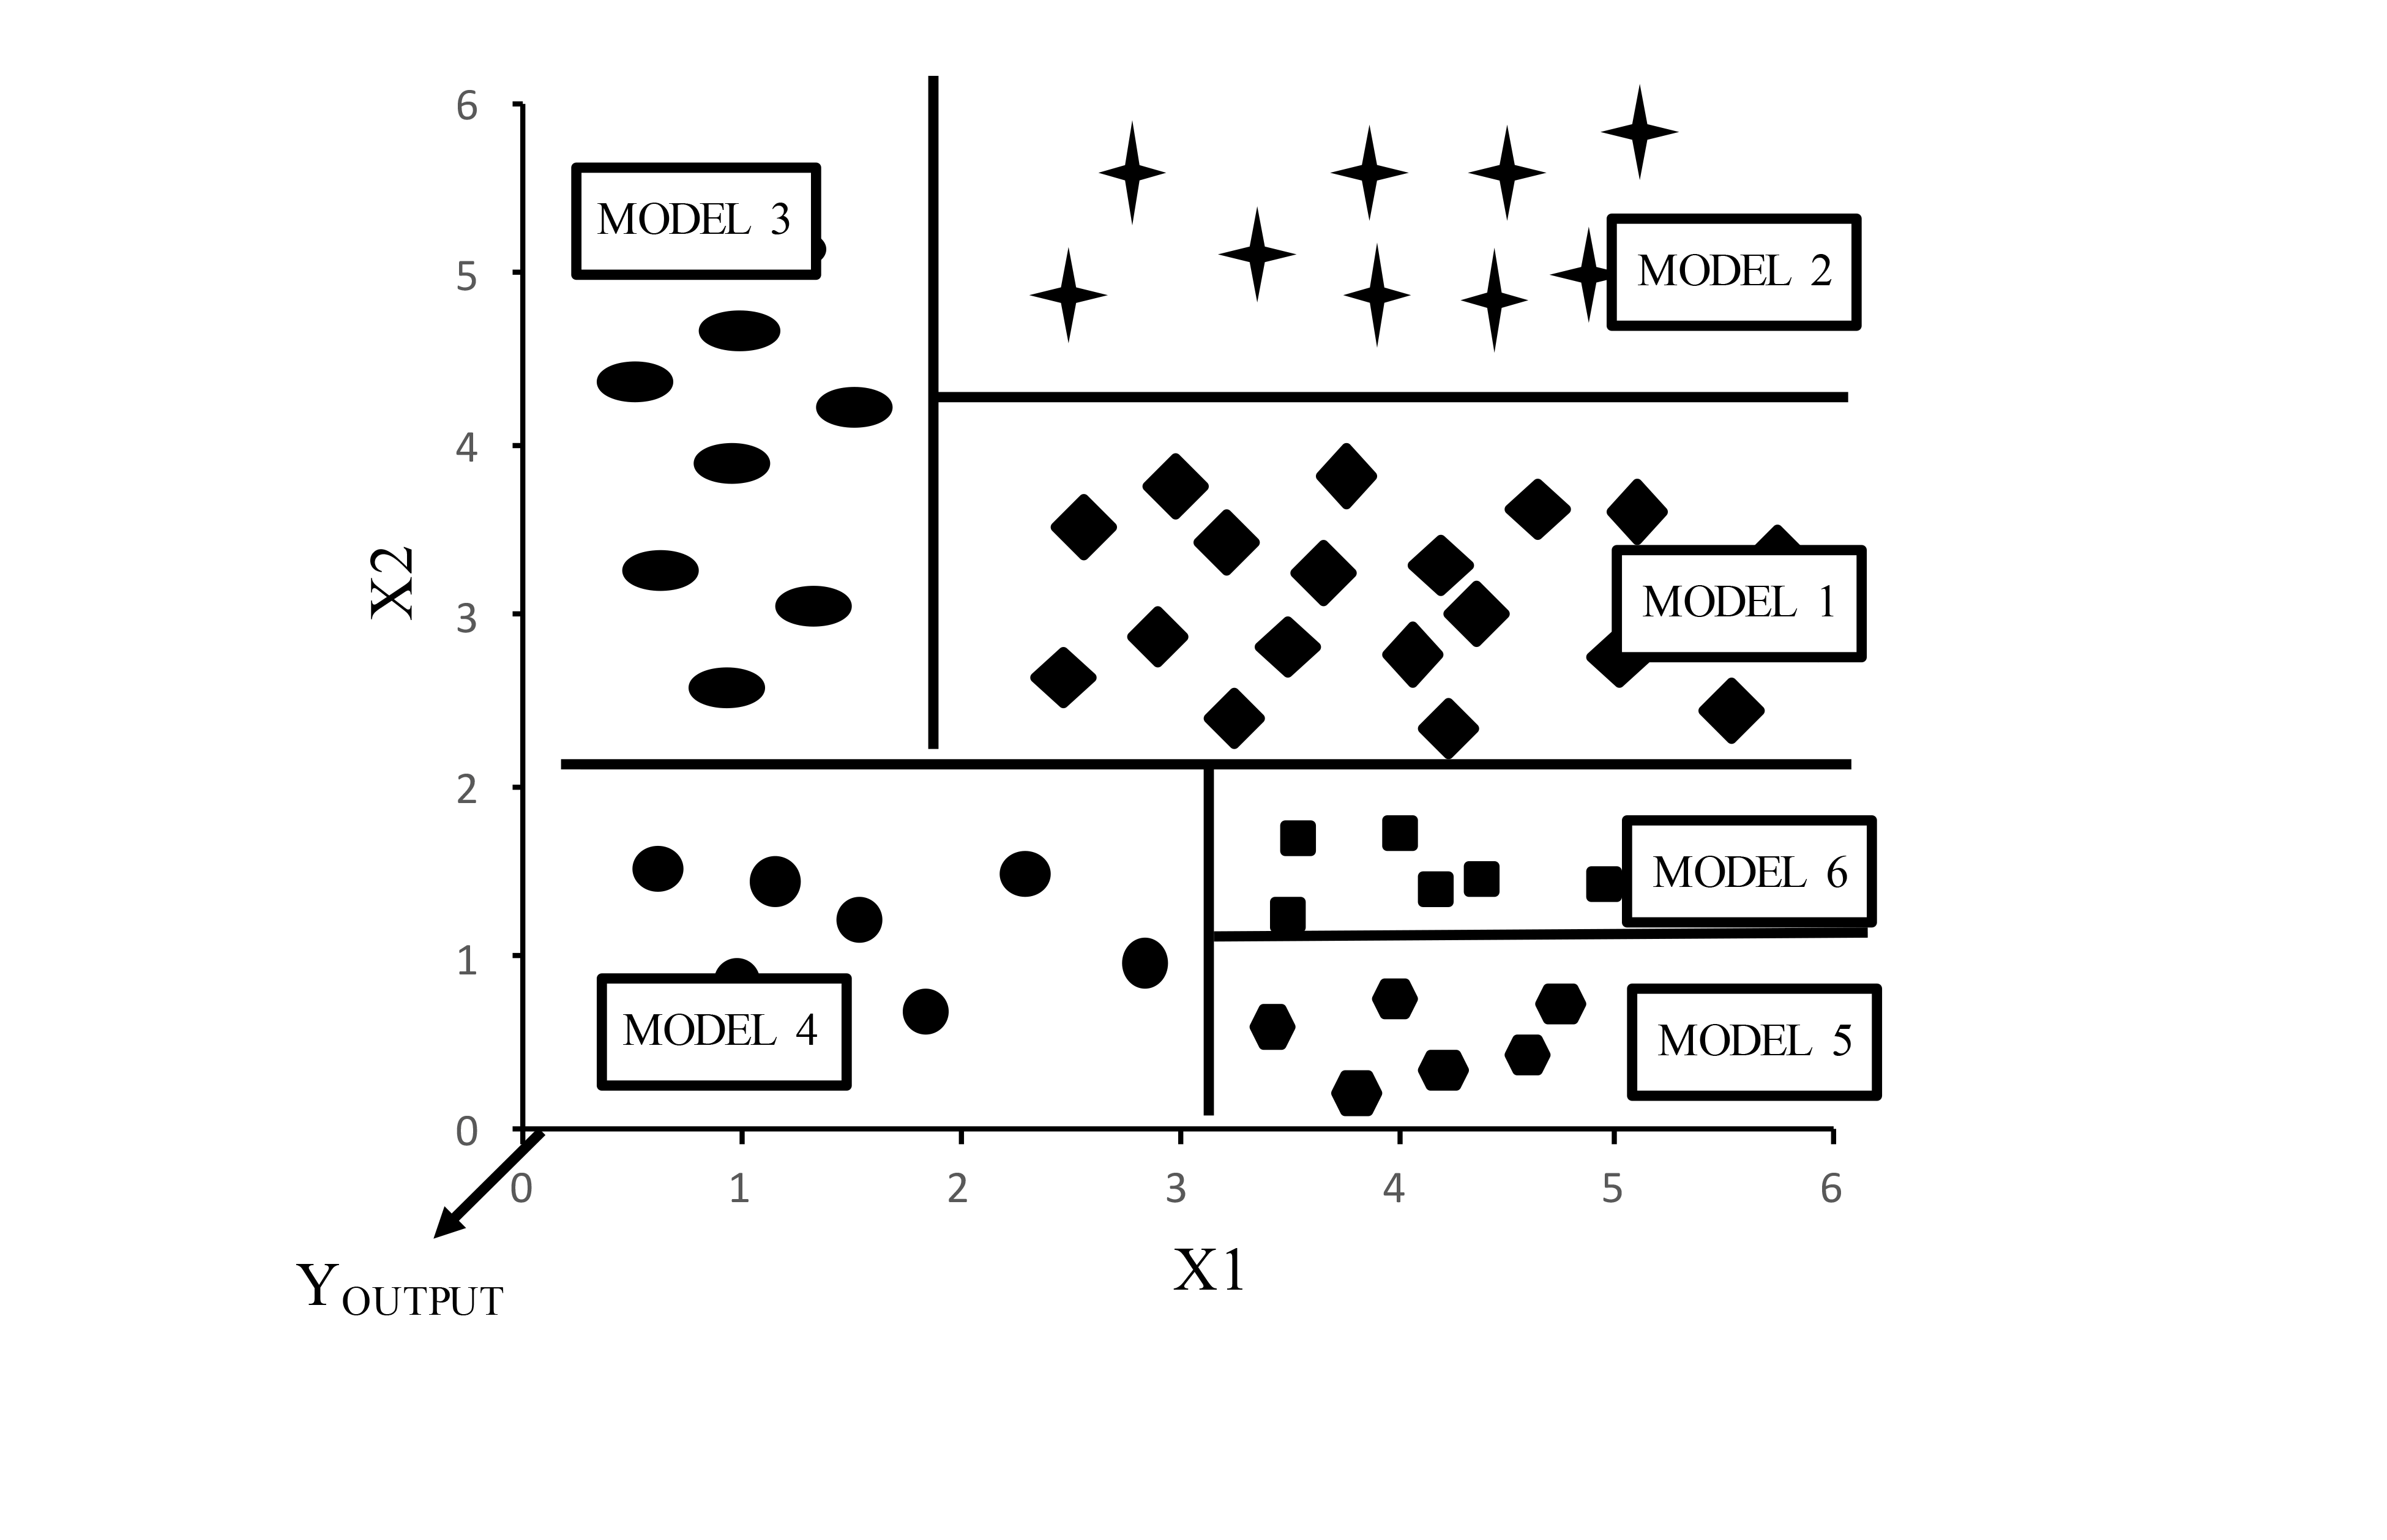
\includegraphics[height=7cm]{splits.png}
% \caption{Splitting of the input space (X1 x X2) by M5' model tree algorithm}
% \label{fig5}
% \end{figure}

% \section{Adding another section}
% You can show a lot of figures together like these Figures \ref{fig61}, \ref{fig62}, \ref{fig63} below.
% \begin{figure} [!htbp]
% \centering    
% \subfigure[Caption1]{\label{fig61}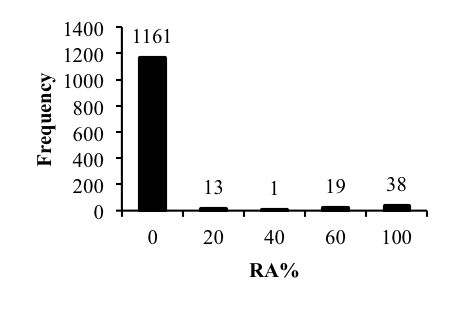
\includegraphics[width=42mm]{data1.png}}
% \subfigure[Caption2]{\label{fig62}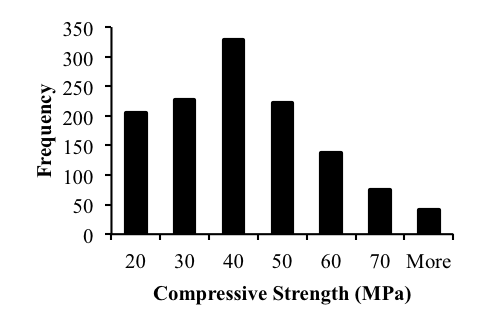
\includegraphics[width=42mm]{data2.png}}
% \subfigure[Caption3]{\label{fig63}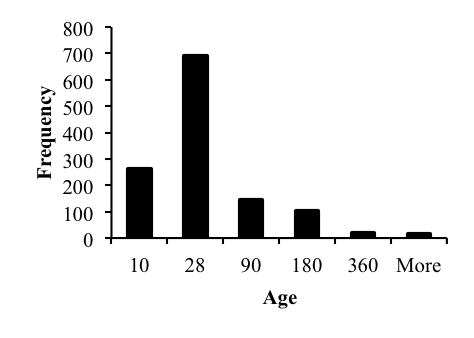
\includegraphics[width=42mm]{data3.png}}
% \caption{Figures sample}
% \end{figure}
% You can add lists into the text like this. 
% \begin{itemize}
% \settowidth{\leftmargin}{{\Large$\square$}}\advance\leftmargin\labelsep
% \itemsep3pt\relax
% \renewcommand\labelitemi{{\lower1pt\hbox{\small$\square$}}}
% \item	Some sample text item 1. 
% \item You may refer to tables \ref{tab1} 
% \item Or figures \ref{fig61}
% \end{itemize}

% Tables can be added like this
% \begin{table}[!htbp]
% \centering
% \caption{Sample table}
% \label{tab1}
% \begin{tabular}{llll}

% \hline
% Column 1 & Column 2 & Column 3       \\\hline
% 1         & Data1 & 13.41179 & 0.9492839 \\
% 2            & Data2 & 13.39824 & 0.9492952\\\hline
% \end{tabular}
% \end{table}




\addtocontents{toc}{\vspace{2em}} % Add a gap in the Contents, for aesthetics

% Solution Architecture - Discuss the solution architecture with reasoning at every step. AG will be there, so be very careful about using the distributed system terms and the solution that you are thinking of. 
% Chapter Template

\chapter{Solution Architecture} % Main chapter title

\label{Chapter 3} % Change X to a consecutive number; for referencing this chapter elsewhere, use \ref{ChapterX}

\lhead{Chapter 3. \emph{Solution Architecture}} % Change X to a consecutive number; this is for the header on each page - perhaps a shortened title

%----------------------------------------------------------------------------------------
%	SECTION 1
%---------------------------------------------------------------------------------------
\section{Assets in the network}

Our blockchain has two native asset types; a liquid asset type and an illiquid asset type. Let’s call the illiquid one BondCoin and the liquid one CashCoin. The blockchain has relatively small number of total coins; lets label this number maxCoins. Each coin is represented by a public-private key pair.

\subsection{BondCoins}

\begin{enumerate}
    \item To start with, a PoW consensus algorithm only mints BondCoins.
    \item After all the BondCoins have been minted, the PoW algorithm subsides and PoS takes over. Owners of BondCoins are the validators.
    \item The private-key of a BondCoin can be used to cast votes during the various phases of the BFT PoS consensus protocol. We can assume the BLS signature aggregation scheme as proposed in the ByzCoin paper for aggregating signatures of BondCoins.
    \item Each BondCoin is of unit denomination and cannot be divided into smaller values.
    \item There is a maturity duration d associated with each BondCoin, say a month. After d time, a BondCoin gets automatically converted into a CashCoin. As an important side benefit, the maturity duration helps in disabling voting rights of dormant BondCoins.
    \item The owner of each BondCoin can also convert it to a CashCoin before maturity but there is a penalty p associated with such a transaction. The convertor derives a value of [CashCoin - p] and p is distributed as fees to other validators.
    \item BondCoins accrue transaction fees for participating in the consensus process. The fees collected during each block are equally distributed among the BondCoins.
    \item BondCoins collectively determine, via consensus, the amount of fees to be charged for processing transactions. This is a key point. We will soon see that for any given number of BondCoins in the system, there is an equilibrium value for the fee amount to which it settles. Transaction validators can also force the fee value to a certain level in order to increase or decrease the number of validators in the system.

\end{enumerate}

\subsection{Benefits of holding BondCoins}

\begin{enumerate}
    \item Storage: Risk free time shifting of value.
    \item Earn Fees: Holders of BondCoin earn a fraction of the transaction fees.
    \item Speculation: BondCoin prices will fluctuate constantly. Speculators that believe that the BondCoin prices are low can buy them.
\end{enumerate}

\subsection{Costs of holding BondCoins}

Holding BondCoins will lead to loss of liquidity. And, to convert them back before maturity would lead to penalty. So, BondCoins act as fixed deposit, you gain interest on them over their maturity period. But you can only take them out once they are fully matured. Otherwise, you will have to compromise with the interest (penalty).

\subsection{CashCoins}

\begin{enumerate}
    \item CashCoins can exist in any denominations and hence are very liquid. You can buy coffee with CashCoin.
    \item Fractions of CashCoin can be accumulated into a unit of CashCoin and further converted into a unit of BondCoin by the owner.
\end{enumerate}

\subsection{Benefits of holding CashCoins}

CashCoins are highly liquid. They can be used in following manner :

\begin{enumerate}
    \item Transactions: People will hold CashCoins to buy goods and services.
    \item Precautions: People will hold CashCoins for contingencies like medical emergencies or the sudden loss in value of a national currency.
    \item Speculation: Speculators that believe that the BondCoin prices are too high can sell them and hold CashCoins instead guarding against possible drops in value of BondCoin.
\end{enumerate}

\subsection{Costs of holding CashCoins}

The price of holding CashCoins is the transaction fees. As these coins could have levied transaction fees while they were not being used. Similar to interests that we gain while keeping our money in a bank.

\section{Market Dynamics}
What we have created with the dual asset types concept is a wonderful interplay between the demand for CashCoins, the demand for BondCoins and the transaction fees. Lets understand the interplay between CashCoins, BondCoins and transaction fees better by noting the costs and benefits of holding either. This is very similar to the interplay between the demand for cash, the demand for bonds and the central bank determined interest rate.

\subsection{Demand Curve for CashCoin}

\begin{figure} [!htbp]
\centering    
\subfigure[Demand Curve for CashCoin]{\label{fig31}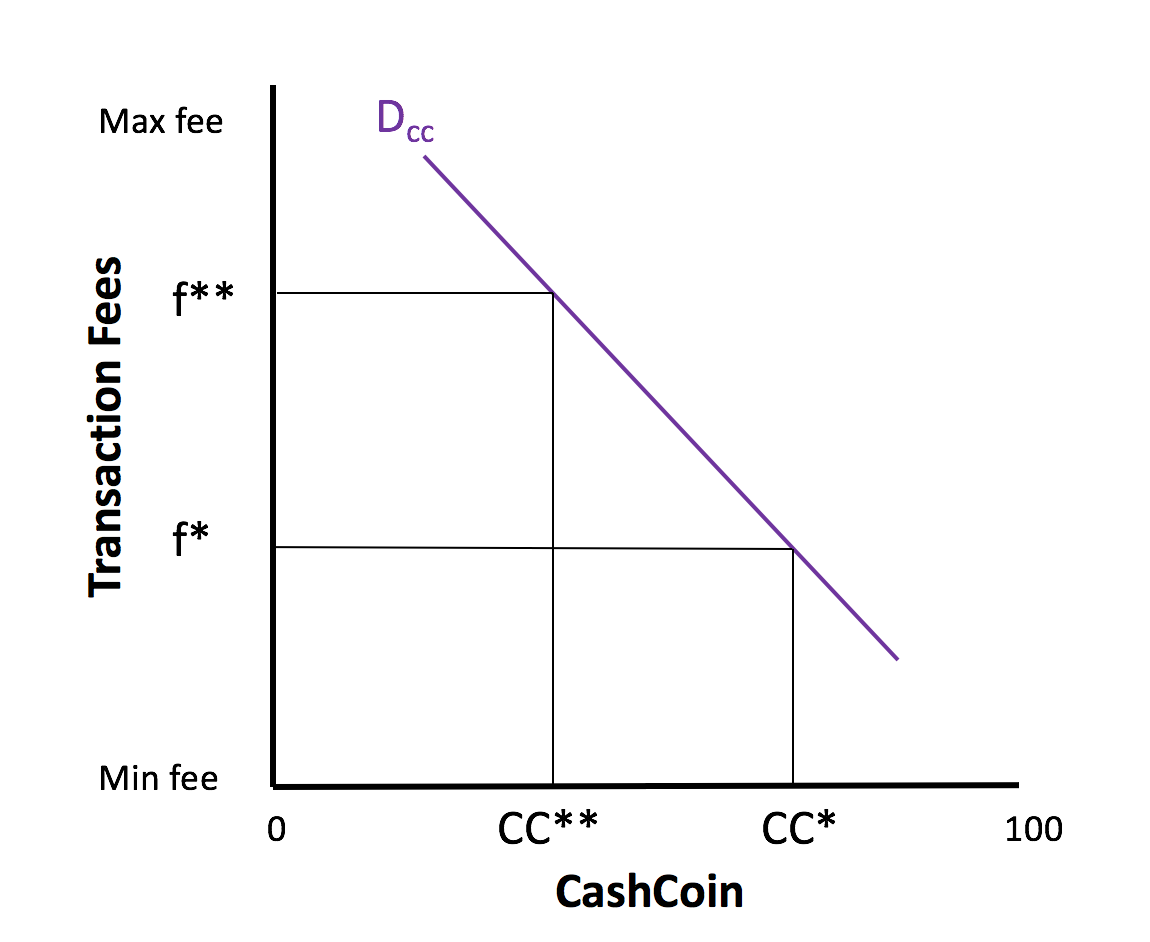
\includegraphics[width=7cm]{dcfc.png}}
\subfigure[Change in demand for CashCoin]{\label{fig32}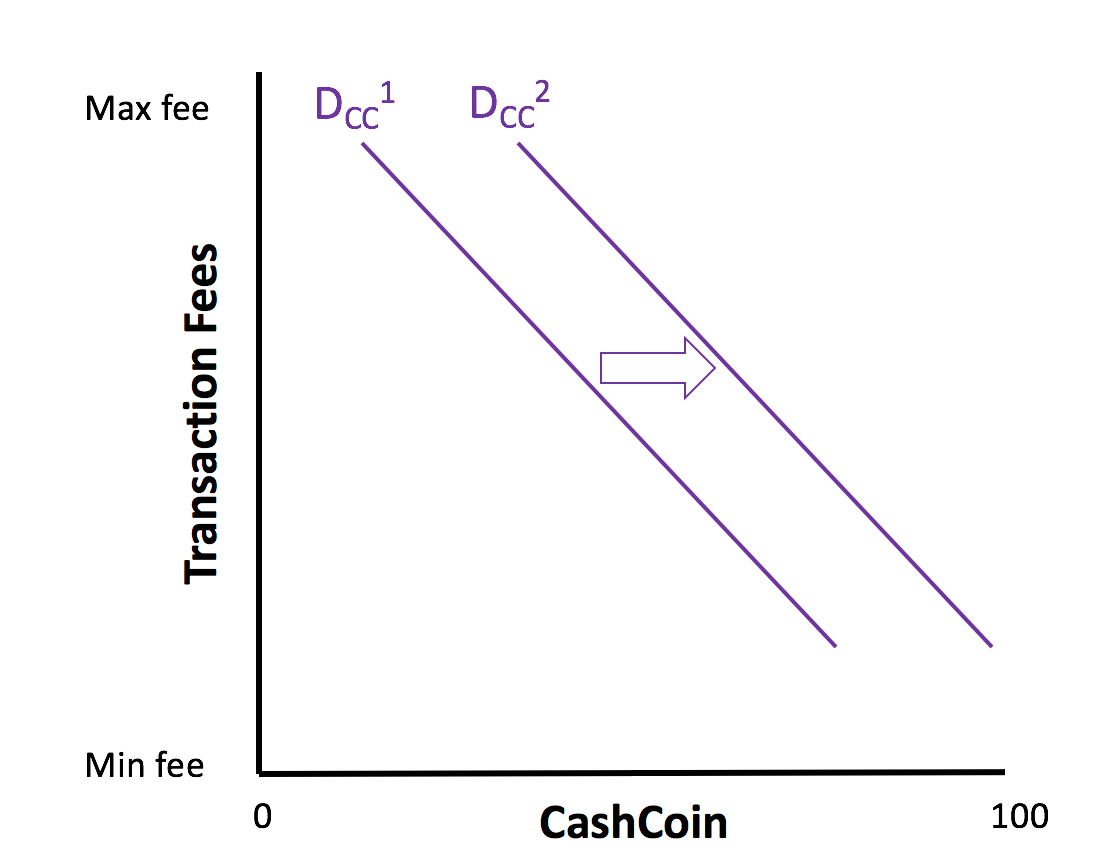
\includegraphics[width=7cm]{cidfc.png}}
\caption{Dynamics of CashCoin}
\end{figure}

The various sources of demand for CashCoins (transactions, precautionary and speculative) will vary negatively with transaction fees. An additional source of demand for CashCoins is from participants wanting lesser decentralization, faster throughputs and lower fees. Let’s label this demand as the higher network performance demand. Lower the fees, higher the demand for CashCoins.

Lets suppose CC** is the total amount of CashCoins at some point in time. I.e., CC** is the supply of CashCoins. Then, the CashCoin market equilibrium will occur at transaction fee f** where the demand meets supply. Now, suppose CashCoin availability increases to CC*, the market equilibrium will occur at transaction fee f* where the demand curve meets the new supply.

\subsection{Change in Demand for CashCoin}

Previously, we have identified 4 sources of demands for CashCoins. i) transactions demand, ii) precautionary demand, iii) speculative demand and iv) higher network performance demand. The various sources of demand for CashCoins can change. For example, during festivals in light of higher retail spending, the transaction demand may rise moving the demand curve as shown in the above figure.

\subsection{Demand Curve for BondCoin}

The various sources of demand for BondCoins (storage, fees and speculative) will vary positively with transaction fees. An additional source of demand for BondCoins is from participants wanting more decentralization and who do not mind paying higher fees. Let’s label this demand as the higher decentralization demand. Higher the fees, higher the demand for BondCoins.

\begin{figure} [!htbp]
\centering    
\subfigure[Demand Curve for BondCoin]{\label{fig33}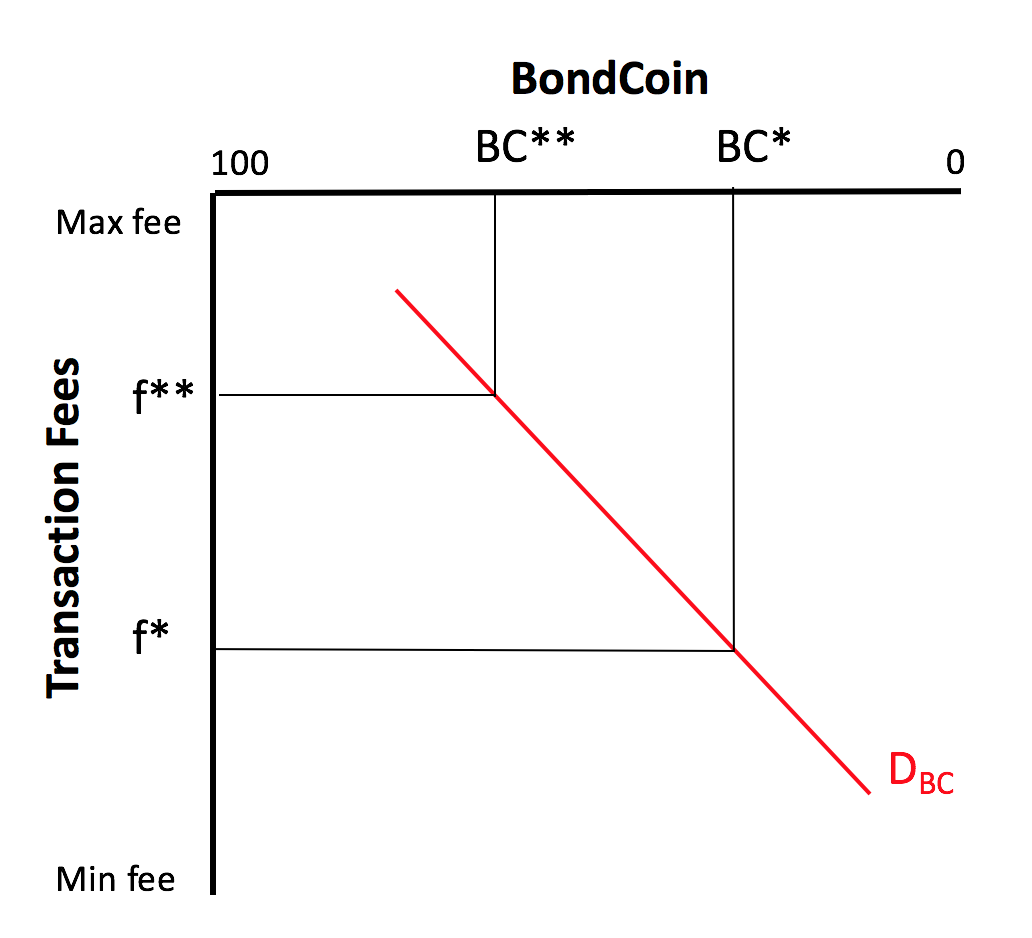
\includegraphics[width=7cm]{dcfb.png}}
\subfigure[Change in demand for BondCoin]{\label{fig34}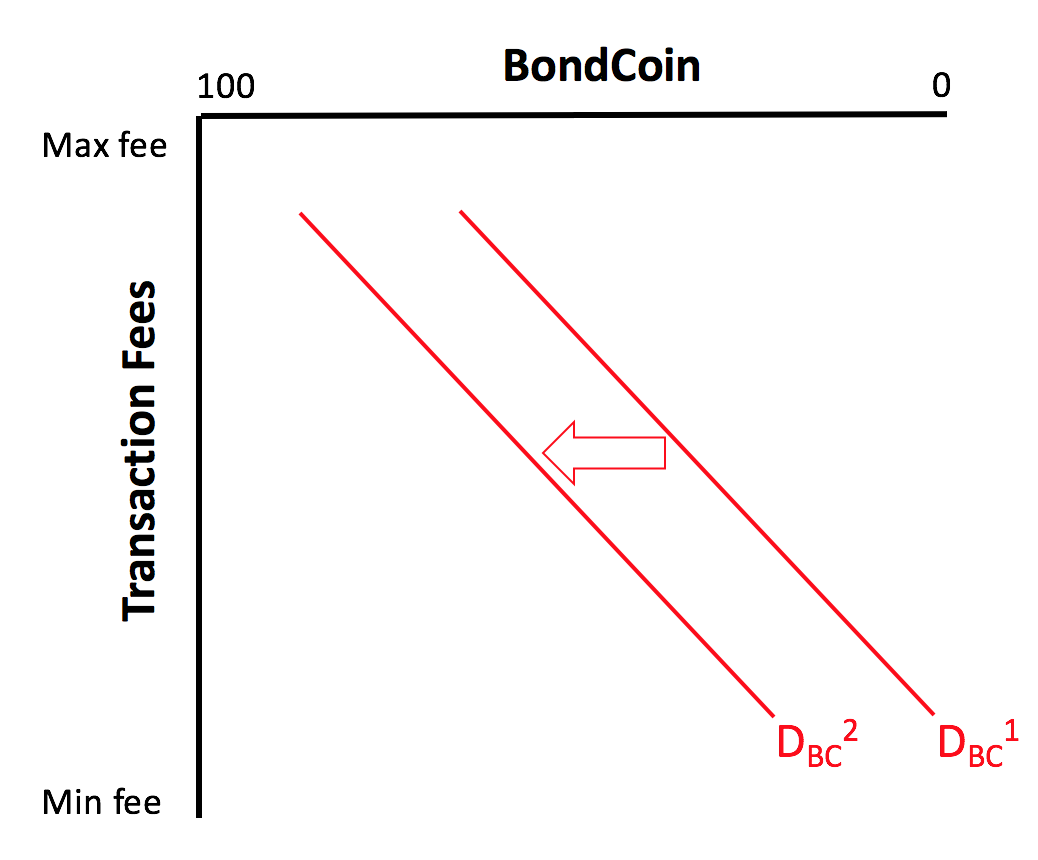
\includegraphics[width=7cm]{cidfb.png}}
\caption{Dynamics of BondCoin}
\end{figure}

Lets suppose BC* is the total number of BondCoins at some point in time. I.e., BC* is the supply of BondCoins. Then, the BondCoin market equilibrium will occur at transaction fee f* where the demand meets supply. Now, suppose BondCoin availability increases to BC**, the market equilibrium will occur at transaction fee f** where the demand curve meets the new supply.

\subsection{Change in Demand for BondCoin}

Previously, we have identified 4 sources of demands for BondCoins. i) storage demand, ii) fees demand, iii) speculative demand and iv) higher decentralization demand. The various sources of demand for BondCoins can change. For example, if the transaction fees increase in anticipation of subdued transaction volumes, the fee demand may rise moving the demand curve as shown in the above figure.

\section{The Common Market Equilibrium}

The supply of BondCoins is simply maxCoins - supply of CashCoins. As shown below, it can be represented by a single line. The supply curve intersects with the demand curves of CashCoin and BondCoin at the same point. This is the common market equilibrium for both CashCoins and BondCoins. There is of course a single fee value f for this common market equilibrium.

\begin{figure}[!htbp]
\centering
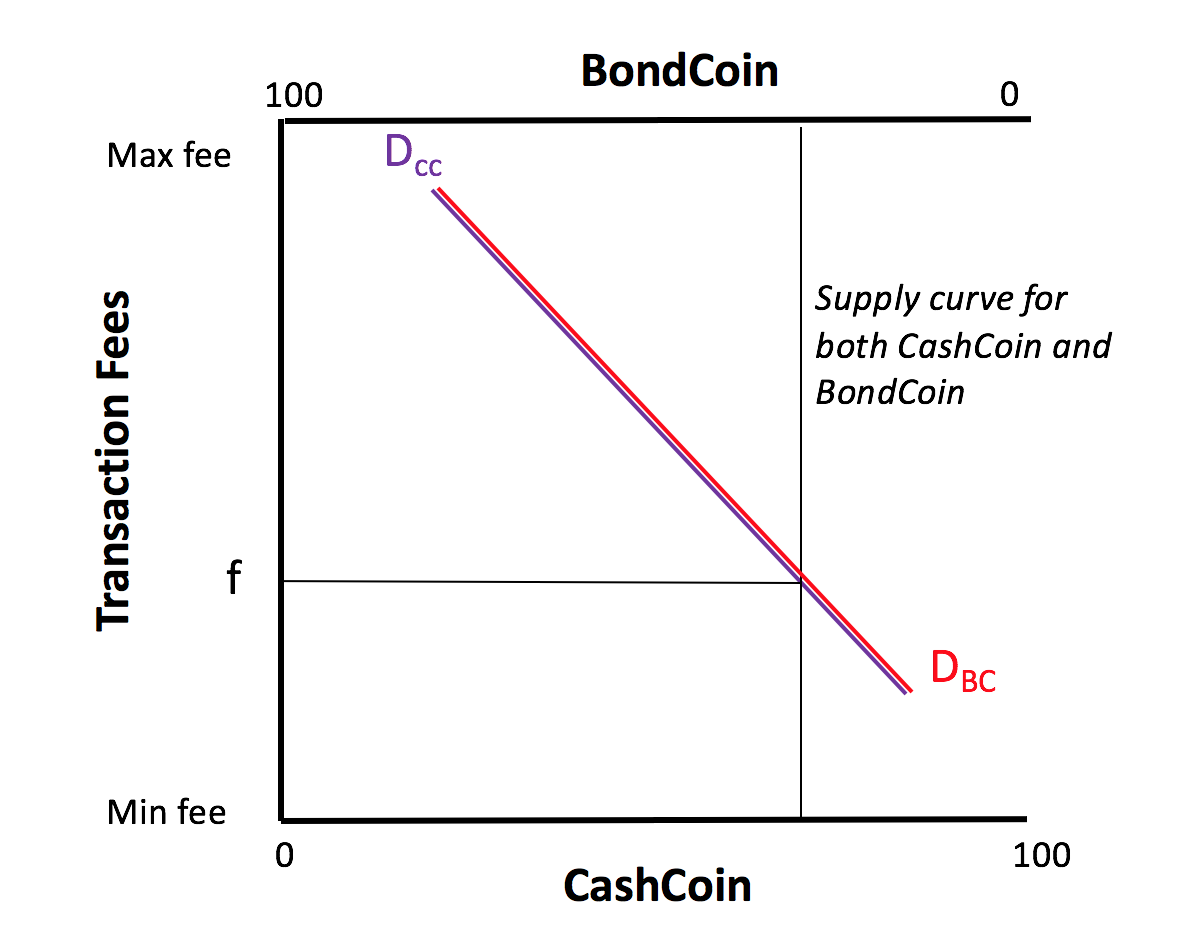
\includegraphics[height=10cm]{tcme.png}
\caption{The Common Market Equilibrium}
\label{fig35}
\end{figure}

This common market equilibrium represents the steady state of the system that respects the aggregate demands and supplies for CashCoin and BondCoin. The number of BondCoins at this equilibrium represent the number of validators in the blockchain.

\section{Modifying More}

Here, we look at how we can change the current system by modifying some crucial parts. For instance, once the BondCoin owners are decided any Byzantine Fault Tolerant protocol can be used to bring a consensus among them.

\subsection{Transaction Functions}

In the existent system, the relationship between BondCoins and transaction fees is linear. This may create problems. If such is the case, then it might happen that BondCoins keep on increasing as transaction fees per BondCoin would be maximum at infinity only. Hence, we need to modify the current relationship between BondCoins and transaction fees.

We define following terms :
\begin{itemize}
    \item Transaction Fees : Fees collected by the Bond Coin owners for working to add a new block to the ledger.
    \item Max transaction fee \%ge : Max \%ge of transaction value that can be collected by the committee members as fees.
    \item Transaction Function : A function that maps number of Bond Coin owners to a transaction fee \%ge. Maximum value can be Max transaction fee \%ge.
\end{itemize}

As we want the number of BondCoin owners to reach equilibrium in the steady state of operation, the transaction function must have a maxima. Hence, the transaction function must look like : 

\begin{figure}[!htbp]
\centering
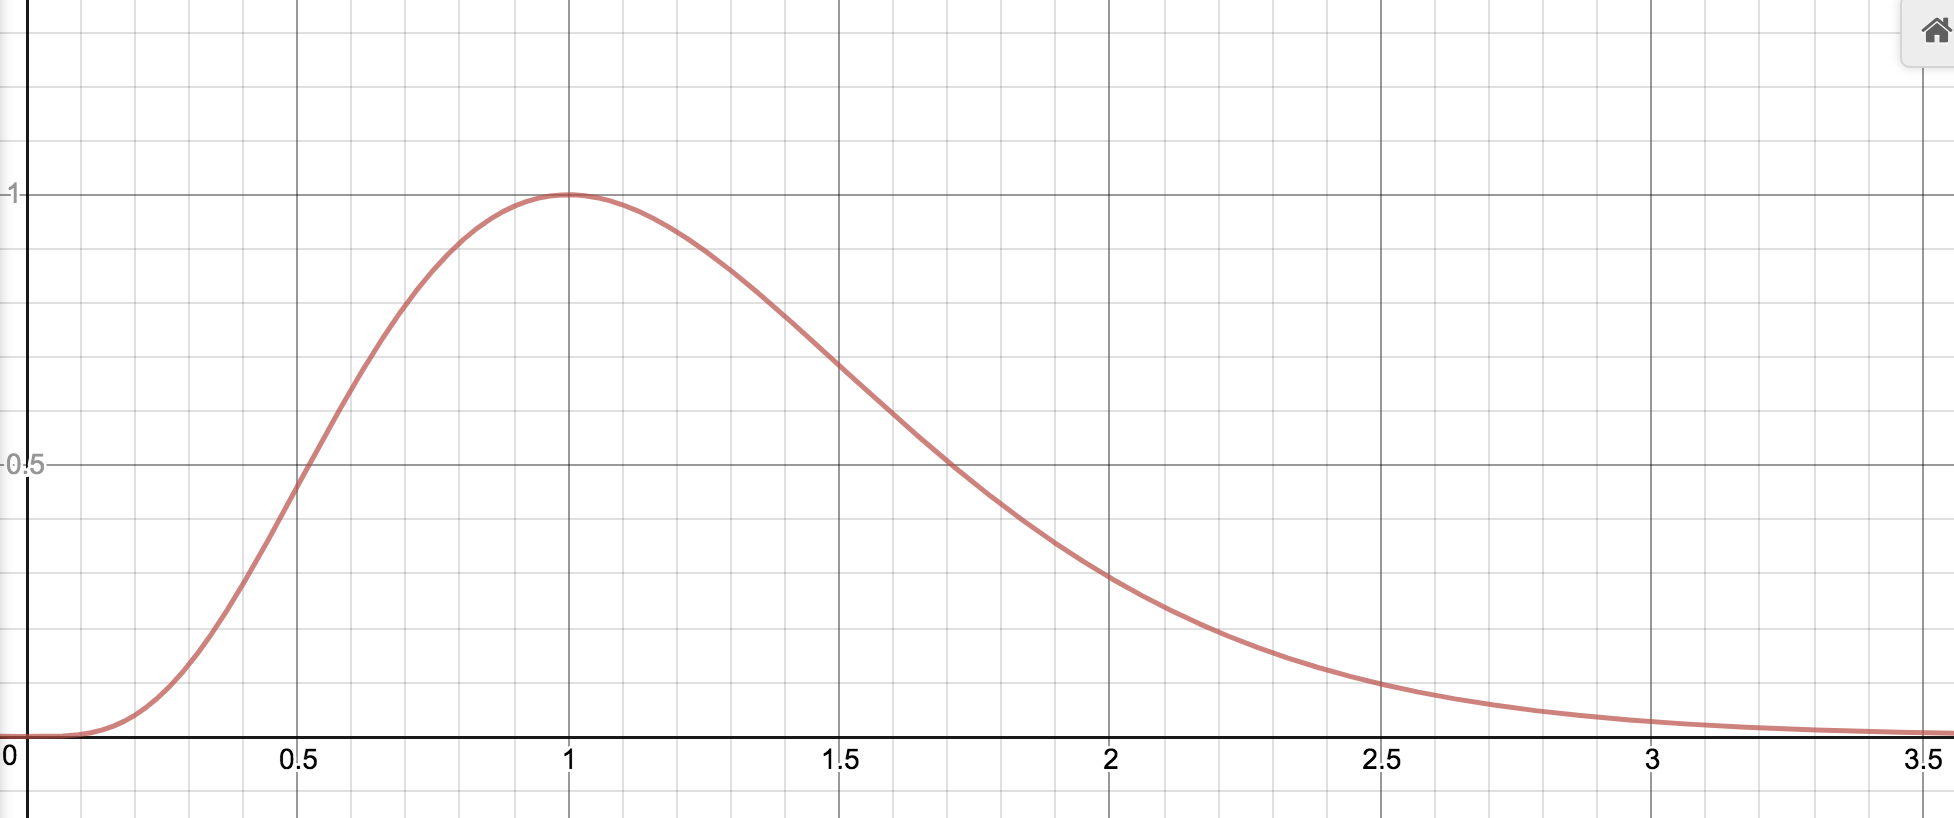
\includegraphics[width=14cm]{Pictures/desiredTF.png}
\caption{Desired Transaction Function}
\end{figure}

Two things that can be adjusted here :
\begin{itemize}
    \item Anchor Point : Denoted by $a$. It is the number of bondcoins when the transaction fees gained by each bondcoin is maximized.
    \item Max Transaction Fee \%ge : Denoted by $m$. It is the maximum transaction fee percentage a user will have to pay in the worst case.
\end{itemize}

We choose the function : $x^n*e^{-x}$ . Analysis of this function shows that the slope gets steeper as we increase the value of n.

\begin{figure}[!htbp]
\centering
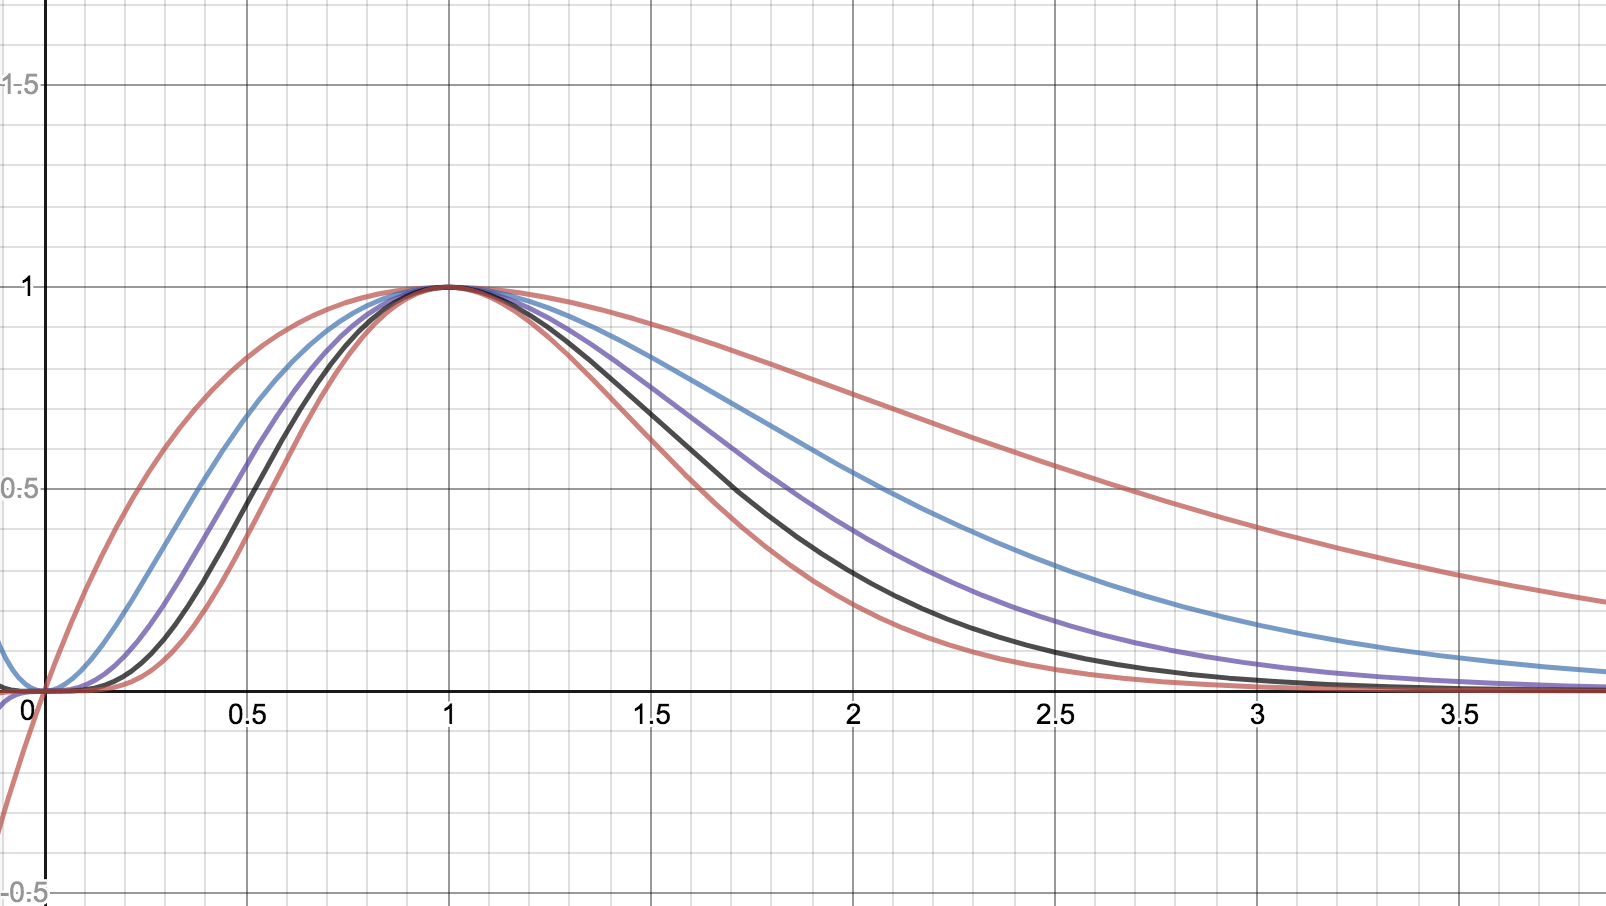
\includegraphics[width=14cm]{Pictures/analyseTF.png}
\caption{Analysis of chosen Transaction Function}
\end{figure}

Now, we can keep $m$ and $a$ fixed or change them depending upon total number of users in the system or total number of active users in the system.

Adjusting the function to give maxima for a bond coin owner at $a$, we get : \\
\centerline{$f(x) = (nx/a)^n*e^{-nx/a}$}

The function of total transaction fee \%ge paid by a user would be : \\
\centerline{$g(x) = x*(nx/a)^n*e^{-nx/a}$}

The maximum value of above function is : \\
\centerline{$({a/n})*(n+1)^{n+1}*e^{-(n+1)}$}

Adjusting the above function to give maximum transaction fee \%ge as m, we get : \\
\centerline{$g(x) = m*((nx/{(n+1)a})^{n+1}*e^{n+1-{nx/a}}$}

Doing same adjustments to $f(x)$, we get : \\
\centerline{$f(x) = m*{1/x}*[nx/{(n+1)a}]^{n+1}*e^{n+1-nx/a}$}

This function reaches maxima at $a$ and the value at maxima is :\\
\centerline{$m*{e/a}*[n/{n+1}]^{n+1}$}

This maximum value is inversely proportional to the value of $a$ and directly proportional to $m$ and is an increasing function with respect to $n$. Hence, more the value of exponent $n$, validators will be able to accrue more fees in the best case.

\subsection{Allocating new BondCoins}

Choosing new Committee members :
\begin{itemize}
    \item We assume that new BondCoin requests keep coming in.
    \item A queue is maintained to keep track of current \& new members
    \item Oldest members appear at the head of the queue \& new members appear at the tail of the queue
    \item There is a logical boundary separating the current members and new members of the queue
    \item The new members become current members only after $s$ blocks has passed
\end{itemize}

We can choose $s$ to be fixed or variable depending upon the number of current committee members.

To filter the incoming BondCoin requests from the users, we keep 2 types of scores :
\begin{itemize}
    \item Cryptocurrency Participation Score or CPS
    \item Transaction Variability Score or TVS
\end{itemize}

\subsubsection{Cryptocurrency Participation Score}

\begin{itemize}
    \item This score gives an idea about how much a user participates in the system (user's participation history)
    \item Initially all users start with a score of threshold b.
    \item We can either use this score as stake for Proof of Stake consensus (requires a random seed) or allow only those users who have a score greater than a threshold b.
\end{itemize}

The CPS at time t depends on CPS at time t-1 and Current Transaction Score (CTS). CTS is a number between 0 to 1.\\
\centerline{$CPS_t = p*CPS_{t-1} + (1-p)*CTS_t$}

Here, we can choose :
\begin{itemize}
    \item p : Probability weightage given to the participation history.
    \item b : Threshold for sending bond coin requests.
\end{itemize}

An insight : Assuming p is 0.99 and b is 0.5, if a user has CPS 0 then it takes it 100 rounds to get to a score of 0.507 with a CTS of 0.8 in each round. From this point, if the user has CTS 0 for 100 rounds then CPS becomes 0.18

Efficient implementation for calculating CPS :
\begin{itemize}
    \item Only needs to be calculated for those users who have done a transaction in the current round.
    \item For those users who aren't taking part in transaction, only last block of transaction needs to be stored and when they send a request for being added in the committee or do a transaction, first the CTS is calculated for the last block using following formula :\\
    If last transaction was done in block $t_1$ and current block is $t_2$ then all the $CTS_t$ for $t = t_1$ to $t_2-1$ would be 0. Hence,\\
    \centerline{$CPS_{t_2} = CPS_{t_1}*p^{t_2-t_1} + (1-p)*CTS_{t_2}$}
\end{itemize}

Current Transaction Score Function : It is a function which gives a score between 0 to 1 based on the total transaction value of a user. Since, this function gives based on transaction value, it should increase steeply in the beginning and go on to saturate so that even low transaction values can contribute.

The candidate functions are : $x^{1/n}$ and $(1-(1-x)^n)^{1/n}$

\subsubsection{Transaction Variability Score}
We can have another score which gives an idea about how many different people does the user transact with and we can use a combination of this and above score to add a new member to committee. This is done to prevent adversarial users from transacting within themselves to gain high CPS. But,
\begin{itemize}
    \item For finding how many different users does a user transact with, we need to keep track of these users (storage constraints) or go back and check the user's transactions when needed (computation constraints)
    \item It might happen that even honest users also transact with a small group of people.
\end{itemize}

Hence, it does not seem a good parameter for selecting allocating new BondCoins.

\addtocontents{toc}{\vspace{2em}} % Add a gap in the Contents, for aesthetics

% Discussion - Discuss the issues that you have got in the system, an idea about how you are trying to solve those. 
% Chapter Template

\chapter{Discussion} % Main chapter title

\label{Chapter 4} % Change X to a consecutive number; for referencing this chapter elsewhere, use \ref{ChapterX}

\lhead{Chapter 4. \emph{Discussion}} % Change X to a consecutive number; this is for the header on each page - perhaps a shortened title

\section{Properties of the system}

Here, we prove the safety and liveness properties of the system.

\subsection{Safety}

Since, we adding users in each round. Therefore, if we use a fixed maturity duration for a bond coin. Then in every round, we have some outgoing users and some incoming users.\\
Also, since the threshold for committing a block is two-thirds of the number of bond coins. Hence, between two consecutive rounds there will be atleast one honest user who has committed the block in that round. Since, the new bond coins are only allocated if the user's hashblock matches with the latest hash. Hence, if an honest user commits a block with bid $x$ and another honest user has committed a block with bid $y$ in the past when it had owned a bond coin, then $y$ must appear in the ledger of $x$.\\
Now, since more than two-thirds of the users are honest and more than two-thirds of the votes are needed for successful commit, hence a block would be committed only if atleast one-half of honest users commit it. And, honest users get consensus only if the block is correct hence the Safety property is guaranteed.

\subsection{Liveness}

Since, more than two-thirds of the users are honest, and a transaction can be accepted within k blocks, hence, it would be picked up by atleast one honest user and broadcasted to others. In case the highest priority block proposer is not an honest user, and the user sends two different sets of blocks then consensus would fail and a new consensus would take place with new priorities. If the highest priority block proposer sends out only one block and doesn't include this transaction then even though this block gets committed there is a high chance that an honest user will include it within k blocks. Hence, liveness property is guaranteed.

\section{Problems in System Design}

Here, we note some of the problems and boundary cases that might occur during the design and execution of the system and we try to give some plausible solutions.

\begin{enumerate}
    \item We know that CashCoins are liquid and can be transferred from one user to another. But, what if a user wants to transfer his voting rights to another user? If this user simply transfers it then he would also have to share the public-private key associated with this coin, but these are digital quantities and can be copied and can lead to the free-rider problem.\\
    Solution : Here, we assume that BondCoins are illiquid and non-transferable. If some user wants to transfer them, then he first has to convert the Coin to CashCoin and send these to the target user who then can convert these back to a BondCoin. This also avoids the free rider problem as when the target user gets his BondCoin, he would also get a new key pair associated with it.
    \item The bond coins are going to be minted using PoW. Once, all the bond coins are minted, the system adopts PoS system. PoW means we are finding some nonce which satisfies some properties, (In case of bitcoin, it had to be less than a given number). But, here the each bond coin is associated with a public and a private key pair which satisfy their own properties. How does the two gets associated?\\
    Solution : Here, the nonce and key-pairs are not related. A user can get a key pair even when PoS has taken over. We use El Gamal Cryptosystem for getting the private-public key pair associated with the BondCoin. This Cryptosystem is based on Elliptic Curve Cryptography (ECDLP) and provides better security with lesser key size. The Base point is common for all users. The private key can be decided by the winner of the current round randomly and based on it a public key can be chosen. But, once its decided, the user cannot change it and has to wait till the BondCoin matures. If he wants to change it then he would have to convert it to CashCoin and then again to BondCoin to choose a new one.
    \item What happens if a user who already owns a BondCoin wins another round while PoW consensus is active?\\
    Solution : If a user wins another round while PoW consensus is active, then he gets to commit that block but the BondCoin that is minted gets added to his account as CashCoin without any penalty. This is done to make sure that each validators has equal voting rights and hence own only one BondCoin with them.
    \item Here we note that PoW algorithm is only for minting bond coins. So, do the users don’t transact till all the bond coins are minted or does the peer minting the next bond coin becomes the leader for that round and commits the block of transactions to the ledger and once all the minting is over, PoS takes over and only those peers can take part in validation who are holding the bond coins?\\
    Solution : Here, we go with the choice that when the PoW consensus is active, the users can still transact and transaction fees are not taken from them. This is done to invite new users to the system and to increase the validators in the system. To incentivise users to participate in the consensus, the BondCoin minted in the current round is paid to the winner of the current round. Note that even after winning once, the users would still want to participate in the consensus to increase the CashCoins in their account.
    \item Each BondCoin comes with a maturity duration d. How is this maturity duration decided? What happens to the keys of the BondCoin once it gets expired and gets converted into CashCoin?\\
    Solution : Currently, this maturity duration is kept as a constant. Eg: 1 month. And, we plan to decide this value emphirically. Each BondCoin comes with a manufacture date, which is stored in the ledger. Once a BondCoin is expired, it gets added as CashCoins to the user account and the keys become useless. This process takes place the first time user transacts after his BondCoin is expired. If he tries to vote using the old keys then his vote is discarded during the expiration check phase.
    \item Since, the CashCoins are not converted automatically to BondCoins, what happens when there is no BondCoin left in the system?\\
    The situation where no BondCoins are left in the system is hard to occur. As the BondCoins in the system decrease, the transaction fees would decrease. In this case, automatically the demand for BondCoins would increase as the few users who are owners of the last few BondCoin would enjoy more shares of the transaction fees by themselves. But, no BondCoin situation can occur only when the last of BondCoins also got matured automatically and no other user converted their CashCoin into a BondCoin before their expiration which would bring the system to a standstill. If there are no BondCoin in the system then there would be no validators in the system and no user would be able to transact and hence the CashCoins in their account would become useless. In this unlikely situation, we suggest that the PoW system is restarted so that the BondCoins in the system can be increased and users can enjoy transactions without paying the fees and do not have to leave the system.
    \item Why is there a penalty for converting BondCoin to CashCoin? How is its amount fixed?\\
    Solution : The BondCoin is like a contract given to user to participate in the validation process during its maturity period. Its like a fixed deposit done in bank, on which you get the interest during the period but you can use the money only after it matures, if you take the money out before it matures then you have to pay a penalty. In a similar way, this penalty is imposed on those users who want to do away with their responsibility of participating in the validation process. The amount is fixed based on the number of BondCoins currently in the system. More the number of BondCoins, more the penalty.

\end{enumerate}

\section{Plausible attacks}

Here, we assume that the block has been prepared and validators are decided, we only need to consider attacks that can be made while committing this block to the ledger.

\begin{enumerate}
    \item Adversary can be the owner of majority of bond coins. Adversary can make multiple accounts with only enough cash coin to convert them into bond coins.
    \item If in response to above, the bond coins are made larger in number then network attacks would be easier. Adversary may be able to slow down the network or partition some nodes.
    \item Instead of buying the bond coins itself, adversary may hack prominent accounts holding bond coins. It's useful as they are gonna be valid for duration d.
\end{enumerate}

\addtocontents{toc}{\vspace{2em}} % Add a gap in the Contents, for aesthetics

% Discussion - Discuss the issues that you have got in the system, an idea about how you are trying to solve those. 
% Chapter Template

\chapter{Distributed Algorithm} % Main chapter title

\label{Chapter 5} % Change X to a consecutive number; for referencing this chapter elsewhere, use \ref{ChapterX}

\lhead{Chapter 5. \emph{Distributed Algorithm}} % Change X to a consecutive number; this is for the header on each page - perhaps a shortened title

\section{Assumptions}

We take the following assumptions for our distributed system :

{
\singlespacing
\begin{itemize}
    \item Each user has a unique id
    \item Each user knows other users
    \item Each user is a node in itself
    \item More than 2/3rd of the users (or specifically the committee members) are honest (non-faulty and form the largest sub) in the system (non-faulty)
    \item New requests for bond coin keep coming in
    \item Each user has a unique public address known to other user while its active
    \item Asynchronous system (Network Faults can happen)
    \item Eventually synchronous system (Eventually all network faults would be resolved)
    \item Reliable connection
    \item Each function is executed atomically
\end{itemize}
}

\section{Abbreviations}

Following are the abbreviations used to denote some fields and classes :
{
\singlespacing
\begin{itemize}
    \item id = User's ID
	\item mt = Transaction Type
	\item sid = Sender's ID
	\item rid = Reciever's ID
	\item t = Timestamp, can also be the id of the last block seen by the user to avoid time conflicts
	\item cc = CashCoin
	\item bc = BondCoin
	\item pk = Public Key of a user
	\item sk = Secret Key / Private Key of a user
	\item val = Transaction amount value that a user wants to send to another user
	\item h = hash obtained on applying a verifiable random function on the message using sk
	\item p = proof for verifying the hash of a message using that user's pk
	\item pa = public address for committee to communicate with this node during consensus
	\item fb = First Block in which a user starts giving consensus
	\item lb = Last Block after which a user stops giving consensus
	\item cps = Cryptocurrency Participation Score
	\item k = The number of blocks till which a transaction is valid. If a transaction is more than 
\end{itemize}
}

\section{Message Types}

Following messages will be exchanged in the system :

{
\singlespacing
\begin{enumerate}
    \item Transfer : Message gossiped by the a node with id sid to send val amount of cashcoins to a node with id rid at timestamp t.
    \begin{verbatim}
Message Transfer
{
    mt
    sid
    rid
    val
    tc
    t
    h
    p
}
    \end{verbatim}
    \item RequestBC : Message requesting to convert cashcoin to bondcoin and become a member of the committee.
    \begin{verbatim}
Message RequestBC
{
    mt
    sid
    pa
    tc
    t
    h
    p
}
    \end{verbatim}
    \item RequestCC : Message requesting to convert bondcoin to cashcoin before maturity.
    \begin{verbatim}
Message RequestCC
{
    mt
    sid
    tc
    t
    h
    p
}
    \end{verbatim}
    \item ChangePK : Message requesting to change pk.
    \begin{verbatim}
Message ChangePK
{
    mt
    sid
    pk // New Public Key
    tc
    t
    h
    p
}
    \end{verbatim}
    \item Join : Message requesting to join the system as a new user. The new id would be mentioned in the next few blocks as confirmation.
    \begin{verbatim}
Message Join
{
    mt
    pk
    tc
    t
    h
    p
}
    \end{verbatim}
    \item BlockCommit : Message broadcasted to give info about a new block.
    \begin{verbatim}
Message BlockCommit
{
    mt  // type of message
    sid // sender id
    block // block list element
    h // hash
    p // proof
}
    \end{verbatim}
\end{enumerate}
}

\section{Variables stored at each node}

{
\singlespacing
\begin{enumerate}
    \item myid = The ID of the user. This is allocated by the system when the user joins for the first time. It is an unsigned number and 0 is reserved for nodes who haven't joined yet. This id is used to index a user's information in the database.
	\item mysk = Private/Secret Key of the user. This is the only private state of the node (same as in algorand) and is used to sign the messages sent by it.
	\item mypk = The public key of the user. This key is advertised by the node so that other nodes can use it to verify its messages, it is unique to a node.
	\item mypa = The public address of the user for other users to send message when it takes part in the consensus. This address is only required when the user requests for a BondCoin.
	\item myfb = The most recent block from which user start participating in consensus
	\item mylb = The most recent block after which user stop participating in consensus
	\item mytc = User's transaction count to distinguish between two of its transaction in the same block, alternative to timestamp.
	\item hblock = Hash of the newest block seen.
	\item nusr = Number of users in the system, used to give id to a new user.
	\item bcuncommitted = Blocks heard but not yet committed. It is a priority queue arranged with respect to bid.
	\item trnuncommitted = Transactions heard but not committed. Transactions are arranged according to last block seen t and no duplicates are stored. The transactions are only stored by prospective BondCoin owners.
	\item nbr = Nearest neighbours in the network, information given by the network. This information is used for Distributed Broadcast of messages.
	\item bcq = A queue of users who have the bond coins and are participating in the consensus or going to participate in the future. No user can be twice in this q at a time. users in the queue can be accessed using their ids. Its like a dictionary but like a priority queue arranged using lb or fb. Implemented using double ended queue.
    Each element of the queue has following definition.
\begin{verbatim}
QueueElement BCUser
{
    id // ID of the user
    pk // Public Key of the user
    pa // Public Address of the user
    fb // first Block giving consensus
    lb // last Block giving consensus
    active // 1 if user is participating in consensus
}
\end{verbatim}
    \item usrd = A dictionary of users which maps a user's id (key here) to all the information about that user.
The values in the dictionary would have following definition
\begin{verbatim}
DictionaryKey id
DictionaryValue User
{
    pk
    lastpa
    cc
    cps
    fb  // the first block from which it joined
}
\end{verbatim}
    \item bcl = A list of blocks which acts as a unified ledger. Each block is a collection of transactions. Each transaction contains the original request and the response given after the consensus. A transaction is included in a block only if it is successful.
Each transaction has the following definition.
\begin{verbatim}
ListElement Transaction
{
    treq // Transaction Request, JSON string
    tres // Transaction Response, JSON string
}
\end{verbatim}
Each transaction can be of following types :
    \begin{enumerate}
        \item Transfer
        \begin{verbatim}
treq = 
{
    mt = `Transfer'
    sid
    rid
    val
    tc
    t
    h
    p
}
tres = 
{
    valfinal // Value transferred to the reciever after 
deducting the transaction fees
}
        \end{verbatim}
        \item RequestBC
        \begin{verbatim}
treq = 
{
    mt = `RequestBC'
    sid
    pa
    tc
    t
    h
    p
}
tres = 
{
    fb
    lb
}
        \end{verbatim}
        \item RequestCC
        \begin{verbatim}
treq = 
{
    mt = `RequestCC'
    sid
    tc
    t
    h
    p
}
tres =
{
    lb
    valfinal // Value to be added to user's account after 
putting fine on it. Fine put on the user as transaction 
fees for converting bc to cc before maturity.
}    
        \end{verbatim}
        \item ChangePK
        \begin{verbatim}
treq = 
{
    mt = `ChangePK'
    sid
    pk // New Public Key
    tc
    t
    h
    p
}
tres =
{
    fb // ID of the block from which the new public key 
would be valid
}    
        \end{verbatim}
        \item Join
        \begin{verbatim}
treq = 
{
    mt = `Join'
    pk
    tc
    t
    h
    p
}
tres =
{
    id // id of the new user
    fb // ID of the block from which the user would be valid
}
        \end{verbatim}
    \end{enumerate}
Each block has the following definition.
\begin{verbatim}
ListElement block
{
    bid // BlockID
    bpid // BlockProposerID
    tlist // List of Transaction Objects
    memlist // List of ids of BondCoin holders who participated 
in this round
    trnfees // Fees earned by each BondCoin owner in this round
    retirelist // List of ids of BondCoin holders who retire 
after this round
    joinlist // List of ids who are given allocated new bondcoins
    nusr // No. of users in the system after accepting new join 
requests in this block
    hprev // hash of previous block
    hq // hash of bcq after applying changes of this block of 
transactions
}    
\end{verbatim}
\end{enumerate}
}

\section{Initialisation}
{
\singlespacing
\begin{enumerate}
    \item myid = 0 or id given by the system when joined the first time
	\item mysk = secret key chosen by me
	\item mypk = public key corresponding to mysk
	\item mypa = public address given by the network to which other users can send messages to communicate with me
	\item mytc = 0 or transaction count of the last transaction
	\item hblock = 0 or hash of the last block in bcl
	\item nusr = 0 or nusr in the last block in bcl
	\item bcq = empty or Queue of users mirrored from a bondcoin holder
	\item usrd = empty or Dictionary of users mirrored from a bondcoin holder
	\item bcl = empty or List of blocks mirrored from a bondcoin holder
	\item bcuncommitted = empty
	\item trnuncommitted = empty
	\item nbr = nearest neighbours in the network, information given by the network
\end{enumerate}
}

\section{Functions}

\subsection{Abstract Functions}
These functions are called by other functions and serve specific tasks.
\begin{enumerate}
    \item Prepare : This function is called before pushing or broadcasting any message. This function sets t, h, p in a message
    \begin{lstlisting}
Abstract Prepare (Message M)
{
    if M.mt in {Transfer, RequestBC, RequestCC, ChangePK, Join} :
        // Can use some mutex while assigning timestamp to avoid 2 transactions getting same timestamp. Instead using tc (transaction count) here. Use mutex while assigning the tc value and incrementing it.
        mytc++
        M.tc = mytc
        M.t = bcl[-1].bid
    M.h = M.p = 0
    (M.h, M.p) = VRF (M, mysk)
}
    \end{lstlisting}
    \item Push : This function sends the message to all the bcowners in the user's queue. Put flag as 1 to send to only active members and 2 to send to all members.
    \begin{lstlisting}
Abstract Push (Message M, flag)
{
    for usr in bcq :
        if flag == 1 and usr.active == 0 :
            break
        if usr.active == -1 :
            continue
        Send M to usr.pa
}
    \end{lstlisting}
    \item Broadcast : This function is used to broadcast a message to the network.
    \begin{lstlisting}
Abstract Broadcast (Message M)
{
    // Implementing distributed broadcast here
    for usr in nbr :
        Send M to usr
}
    \end{lstlisting}
    \item Same : This function is for comparing two messages
    \begin{lstlisting}
Abstract same (treq t1, treq t2)
{
    // Here, we can compare sid but its not generic for all kinds of messages and following four will be enough
    // Added timestamp to distinguish between 2 similar transactions sent in the same block

    // Compare transaction type
    if t1.mt != t2.mt :
        return false
    
    // Compare transaction count
    if t1.tc != t2.tc :
        return false

    // Compare block of transaction
    if t1.t != t2.t :
        return false
    
    // Compare hash
    if t1.h != t2.h :
        return false
    
    // Compare proof
    if t1.p != t2.p :
        return false

    // This means that it is the same transaction, return true
    return true
}
    \end{lstlisting}
    \item Response : This function returns if the transaction was successful.
    \begin{lstlisting}
Abstract Response (Message M)
{
    // Check till k blocks if the transaction has been committed
    for i = M.t + 1 to M.t + k :
        // Check in every TCommit time if the new block has been added to bcl, here TCommit is avg commit time of a block
        while bcl[-1].bid < i :
            wait(TCommit)
        
        // Check in every transaction of the block to find own transaction
        for trn in enumerate(bcl[i].tlist) :
            if same(trn.treq, M) :
                return (true, trn.tres)
    
    // No match means the transaction wasn't accepted
    return (false, null)
}
    \end{lstlisting}
    \item : validUser : This function checks if the user has joined the system ie. it is a valid user or not.
    \begin{lstlisting}
Abstract validUser()
{
    // Check if the user is joined or not
    if myid == -1 :
        raiseError (' User not yet joined in the system ')
}
    \end{lstlisting}
    \item checkBCOwner : This function checks if a usr is BCOwner, pass flag as 1 to search only in current members and flag as 2 to search in all users.
    \begin{lstlisting}
Abstract checkBCOwner(id, flag)
{
    for usr in bcq :
        if flag == 1 and usr.active == 0 :
            break
        if usr.active == -1 :
            continue
        if usr.id == id :
            return true
    return false
}
    \end{lstlisting}
    \item verify : This function verifies a message sent by a user.
    \begin{lstlisting}
Abstract verify(Message M)
{
    if M.mt == Join :
        return VRFVerify(M, M.pk, M.h, M.p) // VRFVerify takes care of hashing when M.h = M.p = 0
    return VRFVerify()
}
    \end{lstlisting}
    \item ExecuteBlock : This function executes the transaction of a new block. If flag is 0 means just verifying the block, if flag is 1 means executing it.
    \begin{lstlisting}
Abstract ExecuteBlock (block, bcq, usrd, flag)
{
    if flag == 0 :

        if block.bid != bcl[-1].bid + 1 :
            return false
        
        // Can also check for bpid and put a hash, proof accordingly here

        // Can also check for priority of block proposer

        // Can make the above two commented checks in the function collecting block proposals itself
        
        // Check if previous hash matches
        if hblock != block.hprev :
            return false

        <Check if memlist matches the current active users in bcq>

        bcq = copy(bcq)
        usrd = copy(usrd)
        input = output = 0
        // Can also check the different memberlist or remove them entirely except memlist

    // Remember to execute RequestCC after RequestBC, can give a pass thru tlist at the end for RequestCC
    for trn in block.tlist :
        if flag == 0 and verify(trn.treq) == false :
            return false
        switch(trn.treq.mt)
            case Transfer :
                usrd[trn.treq.sid].cc -= val
                usrd[trn.treq.rid].cc += trn.tres.valfinal
                if flag == 0 :
                    if usrd[trn.treq.sid].cc < 0 :
                        return false
                    input += val
                    output += trn.tres.valfinal
            
            case RequestBC :
                usrd[trn.treq.sid].cc -= 1
                bcu = newBCUser
                bcu.id = trn.treq.sid
                bcu.pk = usrd[bcu.id].pk
                bcu.pa = trn.treq.pa
                bcu.fb = trn.tres.fb
                bcu.lb = trn.tres.lb
                bcu.active = 0
                bcq.push(bcu)
                if flag == 0 :
                    if usrd[trn.treq.sid].cc < 0 :
                        return false
                    input += 1
                    output += 1
            
            case RequestCC :
                bcq[trn.treq.sid].active = -1
                usrd[trn.treq.sid].cc += trn.tres.valfinal
                if flag == 0 :
                    input += 1
                    output += trn.tres.valfinal
            
            case ChangePK :
                usrd[trn.treq.sid].pk = trn.treq.pk
            
            case Join :
                usrd[trn.tres.id] = new User
                usrd[trn.tres.id].pk = trn.treq.pk
                usrd[trn.tres.id].lastpa = 0
                usrd[trn.tres.id].cc = 0
                usrd[trn.tres.id].cps = thres // here thres is the threshold
                usrd[trn.tres.id].fb = trn.tres.fb
    
    if flag == 0 :
        output += len(memlist)*block.trnfees
        if input != output :
            return false
        
        if len(usrd.keys) != block.nusr :
            return false

    // Add fees to members account
    for id in memlist :
        usrd[id].cc += block.trnfees
    
    // Pop retired members from bcq
    while bcq != empty and bcq.head.lb == bcl[-1].bid :
        bcq.pop()
    
    if flag == 0 :
        hq = hash(bcq)
        if hq != block.hq :
            return false
        return true
    
    // Means flag = 1
    hblock = hash(block)
    nusr = block.nusr
    
}
    \end{lstlisting}
\end{enumerate}

\subsection{Threads}
These functions run independently and may not be atomic.
\begin{enumerate}
    \item Sentinel : This thread runs at the start and tries to get user updated with the latest blocks.
\begin{lstlisting}
Thread Sentinel ()
{
    // run at all times except stops only when user goes offline

    time.reset()
    while(true) :
        
        // Resync if its past resynchronisation period
        if time.gone() > tresync :
            < Explicitly get missing blocks from other users and put it in bcuncommitted and broadcast them too >
            time.reset()

        
        // Commit the uncommitted block if any
        while bcuncommitted != empty and bcuncommitted.head.bid == bcl[-1].bid + 1 : // Here, in case of a bcl empty would need to add another condition, instead either put a dummy block at the start of bcl with id 0 or replace bcl[-1].bid with len(bid), if going with the former can also get the genesis block as a response to the Join message.
            bcl.append(bcuncommitted.head)
            bcuncommitted.pop()
            ExecuteBlock(bcl[-1], bcq, usrd, 1)
        
        // Listen for new message
        M = Listen() 

        // Verify only if not a new user
        if bcl != empty :
            verify(M)

        // Commit Message
        if M.mt == BlockCommit :
            
            // Already updated
            if bcl[-1].bid >= M.block.bid :
                continue
            else :
                bcuncommitted.push(M.block)

                // Only broadcast further if in the network
                if myid != 0 :
                    M.sid = myid
                    Prepare(M)
                    Broadcast(M)

        else if M.mt in {Transfer, RequestBC, RequestCC, ChangePK, Join} :
            // If I am a member
            if bcl[-1].id < mylb :
                trnuncommitted.push(M) // push removes duplicates and puts in the correct position in the queue, it also removes a transaction if already committed using function Response, and removes those which are already expired

            // If I am not an active member ignore
            else :
                continue

                
}
\end{lstlisting}
    \item Participate : This thread runs for the time the user has to participate in the consensus.
\begin{lstlisting}
Thread Participate()
{
    // mylb takes care that I am a member, for voting will also check if an active member, in normal operation the thread itself will destroy
    while bcl[-1].bid < mylb :
        <remove transactions from truncommitted who are accepted and those for which this block is the last hope and still they are not valid>
        
        // Take part only if in next block we are an active bcowner
        if bcl[-1].bid + 1 >= myfb :
            if <Proof of stake/current block makes me a proposer> :
                <Validate the transactions seen so far>
                <Propose a block>
                <Put priority>
                <Push it to the current active members>
                <Add it to own proposal list>
            
            while <proposal time> :
                <pop a new proposal>
                <check the validity of proposal>
                <put it as this round's block if highest priority> 

            <vote for the highest proposal seen>

            while <voting time> :
                <pop a vote>
                <add the vote>
                <see if the votes for a particular block exceeds 2/3rds of the total votes>
                <if it does commit this block and broadcast>
                <break> 

        <wait till new block is committed>
        <if not committed within some time restart consensus>

    destroy truncommitted
    Stop this thread
}
\end{lstlisting}
\end{enumerate}

\subsection{Public Functions}
These functions can be called directly by the user or are called depending on the events triggered by actions of the user.
\begin{enumerate}
    \item Wakeup : This function is called when the node boots up.
    \begin{lstlisting}
Wakeup () :
    Start thread Sentinel()
    \end{lstlisting}
    \item Shutdown : This function is called when the node is shutting down.
    \begin{lstlisting}
Shutdown () :
    If myid in bcq :
        <Push RequestCC>
        <Wait till the request is accepted>
    Stop thread Sentinel()
    \end{lstlisting}
    \item Transfer : This function is called by the user when it wants to transfer money to another user.
    \begin{lstlisting}
Transfer (rid, val)
{
    // Check if the user is joined or not
    validUser()
    
    // Check if reciever is valid or not
    if rid > nusr :
        raiseError (' Reciever is not valid ')

    // Check if val is valid
    if val > usrd[myid].cc :
        raiseError (' Not enough cashcoins to send ')

    // Prepare the message for sending
    mtransfer = new Message
    mtransfer.mt = Transfer
    mtransfer.sid = myid
    mtransfer.rid = rid
    mtransfer.val = val

    // Set tc, t, h, p
    Prepare (mtransfer)

    // Send the message to all the bcowners including those who have not yet started
    Push (mtransfer, 2)

    // Get response for the transaction
    (success, tres) = Response (mtransfer)

    // As the user's own accounts will also be handled in a general way, no use of tres here

    // return if the transaction was successful
    return success
}
    \end{lstlisting}
    \item RequestBC : This function is called by the user when it wants to participate in the consensus
    \begin{lstlisting}
RequestBC ()
{
    // Check if the user is joined or not
    validUser()

    // Check if the user has enough cashcoins
    if 1 > usrd[myid].cc :
        raiseError (' Not enough cashcoins to convert to bondcoin ')

    // Prepare the message for sending
    mrequestBC = new Message
    mrequestBC.mt = RequestBC
    mrequestBC.sid = myid
    mrequestBC.pa = mypa

    // Set tc, t, h, p
    Prepare (mrequestBC)

    // Send the message to all the bcowners including those who have not yet started
    Push (mrequestBC, 2)

    // Get response for the transaction
    (success, tres) = Response (mrequestBC)

    if success :
        // Set myfb and mylb
        myfb = tres.fb
        mylb = tres.lb
        create tnuncommitted
        start thread Particpate()

    // return if the transaction was successful
    return success
}
    \end{lstlisting}
    \item RequestCC : This function is called by the user when it wants to convert its bondcoin before maturity.
    \begin{lstlisting}
RequestCC ()
{
    // Check if the user is joined or not
    validUser()

    // Check if the user is in bcq
    if not checkBCOwner(myid, 2) :
        raiseError (' User not in BCOwner queue ')

    // Check if the user holds bc now
    if (bcl[-1].bid+1) == lb :
        raiseError (' User in BCOwner queue but this is last block ')
    
    // Prepare the message for sending
    mrequestCC = new Message
    mrequestCC.mt = RequestCC
    mrequestCC.sid = myid
    
    // Set tc, t, h, p
    Prepare (mrequestCC)

    // Send the message to all the bcowners including those who have not yet started
    Push (mrequestCC, 2)

    // Get response for the transaction
    (success, tres) = Response (mrequestCC)

    if success :
        // Set mylb
        //myfb = tres.fb
        mylb = tres.lb
        destroy trnuncommitted // can also just clear it
        Stop Thread Participate()

    // return if the transaction was successful
    return success
}
    \end{lstlisting}
    \item ChangePK : This function is called by the user when it wants to update its public key.
    \begin{lstlisting}
ChangePK (newpk)
{
    // Check if the user is joined or not
    validUser()

    // Prepare the message for sending
    mchangePK = new Message
    mchangePK.mt = ChangePK
    mchangePK.sid = myid
    
    // Set tc, t, h, p
    Prepare (mchangePK)

    // Send the message to all the bcowners including those who have not yet started
    Push (mchangePK, 2)

    // Get response for the transaction
    (success, tres) = Response (mchangePK)

    if success :
        // Set mypk
        mypk = newpk

    // return if the transaction was successful
    return success
}
    \end{lstlisting}
    \item Join : Called by a user to join the system for the first time. The bcowners check if the public key provided by the user is unique or not. If it is the user is given a unique id after which the user can start using the system. On success, the user would start mirroring the previous blocks, queue of users and dictionary of users from any member of the system.
    \begin{lstlisting}
Join ()
{
    // Can check if the user already exists but it might happen that same client wants to join as multiple user so we allow it here.

    // Prepare the message for sending
    mjoin = new Message
    mjoin.mt = Join
    mjoin.pk = mypk
    
    // Set tc, t, h, p
    Prepare (mchangePK)

    // Send the message to all the bcowners including those who have not yet started
    Push (mjoin, 2)

    // Get response for the transaction
    (success, tres) = Response (mchangePK)

    if success :
        // Set myid
        myid = tres.id

    // return if the transaction was successful
    return success
}
    \end{lstlisting} 
\end{enumerate}

\addtocontents{toc}{\vspace{2em}} % Add a gap in the Contents, for aesthetics

% Conçlusion and Future Works. 
% Chapter Template

\chapter{Conclusion and Future Works} % Main chapter title

\label{Chapter 6} % Change X to a consecutive number; for referencing this chapter elsewhere, use \ref{ChapterX}

\lhead{Chapter 6. \emph{Conclusion and Future Works}} % Change X to a consecutive number; this is for the header on each page - perhaps a shortened title

In this report, we saw how the number of validators for a POS system can be dynamic and may be determined by the market parameters. The POS systems were better than POW systems because they don't waste computational power in redundant tasks but POS systems itself has some drawbacks. The proposed system tries to solve some of these drawbacks. The crux of the proposed system lies in the fact that all the validators are given equal voting rights so that adversary is also ripped off of the probabilistic advantage of gaining the control of the system which is prevalent in the recently proposed systems such as Algorand. In this system, gaining half the currency of the system is not enough for the adversary. He must have control over more than half of the BondCoins i.e. more than half of the computation power. And, as these BondCoins come with an expiry, the task of the adversary becomes more difficult.

In future we would like to achieve the following objectives :
\begin{enumerate}
    \item We would like to explore how the system is affected if the maturity duration of a BondCoin is variable
    \item We would like to devise a method to ensure that a minimum number of validators are always there in the network at a given point of time
    \item We would like to explore how the system is affected if the BondCoin is also quantized. For eg : a group of users can combine their CashCoins to get one BondCoin. What would be the final vote of such a group of users?
    \item Till now, we have assumed that all the validators remain active all the time. We would like to explore what happens if some of the validators crash or go offline.
    \item We would like to tackle the geographical scalability of POS protocols and devise a solution for it.
    \item We would like to scale the implemented system and run benchmark tests on it.
    \item We would like to explore how charging fees for conversion of CashCoin to BondCoin affects the economy of the system.
    \item We would like to prove the system's correctness under weaker assumptions.
    \item Change the relation between BondCoins and transaction fees and analyse the new system.
\end{enumerate}

\addtocontents{toc}{\vspace{2em}} % Add a gap in the Contents, for aesthetics

% Conçlusion and Future Works. 
% Chapter Template

\chapter{Related Works} % Main chapter title

\label{Chapter 7} % Change X to a consecutive number; for referencing this chapter elsewhere, use \ref{ChapterX}

\lhead{Chapter 7. \emph{Related Works}} % Change X to a consecutive number; this is for the header on each page - perhaps a shortened title

In this section, we see what other kinds of protocols have been proposed to solve the age old state machine replication problem.

\section{Bitcoin}

The protocol on which the cryptocurrency Bitcoin is transacted, this was the earliest of the blockchain protocols. It follows a Proof of work consensus wherein nodes compete among themselves to solve a hard problem. And, whoever solves the problem gets to mine the next block and is accordingly rewarded. The protocol is permissionless that is any user can join and completely decentralized as there is no central authority validating the transactions.

% \begin{itemize}
%     \item It’s a public blockchain, i.e. permission-less, where anyone can join.
%     \item The underlying technology components are cryptographic hash function, digital signature, private-and-public key encryption, peer-to-peer (P2P) network, and proof of work (POW) consensus algorithm.
%     \item The protocol allows users to conduct non-reversible transactions without having to explicitly trust a third-party.
%     \item Every node has the complete information on the blockchain, making the network a decentralized one.
%     \item Transactions contain unique transaction ID, input Bitcoin address, the number of Bitcoins to be transferred, and the output Bitcoin address of the recipient.
%     \item The transaction making process involves the initiator of the transaction, and ‘miner’, i.e. combination of special-purpose software, powerful hardware, and their user. The transaction initiator pays transaction fees to the miner, who tries to include the transaction in the next block. A block is processed in every 10 minutes, and the transactions included in that are then recorded in the blockchain. Creating a new block requires not only the transaction information of the current transaction, but also a reference to the last recorded block. The last recorded block isn’t known, and the miner needs to solve a complex cryptographic puzzle to find it, and this essentially involves a large number-crunching operation done at high-speed. For this, the miner needs to try one number after another, which requires high computing power. Majority of the participating nodes must approve the transaction. Since this is a decentralized network, it isn’t possible for anyone to capture majority of the computing power on the network, thus making the network very secure. Thus, while POW mining ensures high security of blockchain, it’s also computing-power-intensive, and requires high amount of energy.
%     \item The transaction making process involves the initiator of the transaction, and ‘miner’, i.e. combination of special-purpose software, powerful hardware, and their user. The transaction initiator pays transaction fees to the miner, who tries to include the transaction in the next block. A block is processed in every 10 minutes, and the transactions included in that are then recorded in the blockchain. Creating a new block requires not only the transaction information of the current transaction, but also a reference to the last recorded block. The last recorded block isn’t known, and the miner needs to solve a complex cryptographic puzzle to find it, and this essentially involves a large number-crunching operation done at high-speed. For this, the miner needs to try one number after another, which requires high computing power. Majority of the participating nodes must approve the transaction. Since this is a decentralized network, it isn’t possible for anyone to capture majority of the computing power on the network, thus making the network very secure. Thus, while POW mining ensures high security of blockchain, it’s also computing-power-intensive, and requires high amount of energy.
%     \item While the consensus mechanism requiring majority approval rules out foul play, it also creates scalability issues, since every node must load entire information on blockchain and participate in the transaction validation process. Bitcoin blockchain has recently implemented ‘Segregated Witness’ (SegWit) technology, which bypasses the limitation on block size, and separates signature information from the transaction data, to improve scalability of the network.
% \end{itemize}

\section{Ethereum}

Ethereum blockchain has many similarities with Bitcoin protocol, for e.g.: It’s a public, permission-less blockchain; It uses the same technological backbones, for e.g. cryptographic hash function, private-and-public key encryption, P2P network, etc; POW consensus algorithm is used; There’s a native cryptocurrency, called Ether. Ether has the second highest market cap, behind only Bitcoin.

However, unlike Bitcoin, which was built for allowing crypto payment transactions over a decentralized network, Ethereum was designed with much larger objectives in mind. Ethereum provides a blockchain platform, using which developers can launch their own blockchain projects, including their own cryptocurrencies. The platform, commonly called as ‘Ethereum Virtual Machine’ (EVM), has been used to launch over 1,000 DApps. Famous cryptocurrency projects such as VeChain and OmiseGo have been launched using EVM.\\
Smart contracts make this possible. Smart contracts are pieces of code, which allows execution of legal functions, for e.g. taking control of an entity based on certain conditions, and transferring crypto tokens based on fulfilling required conditions. Smart contracts on the Ethereum platform are codes using Ethereum’s proprietary language Solidity, which is inspired by C++, Java, Python and JavaScript.\\
DApps are applications where the backend code runs on a decentralized blockchain, and comprises of smart contracts. Ethereum has made wider adoption of blockchain possible, because of EVM, smart contracts and DApps.\\
Ethereum also provides a way for the user to specify how much computing power will be expended for a transaction, by using a measure of processing power, called ‘Gas’. The user can specify a gas limit. If a transaction remains within that limit then it’s executed, however, if it exceeds the limit, then the changes are reverted. Simple payment transactions require less gas, whereas more complex operations, such as deployment of smart contracts, require more gas.

\section{Ripple Protocol}
Ripple protocol uses many of the features of Bitcoin or Ethereum, such as decentralized design, cryptographic hash functions, P2P network, and private-and-public key encryption. However, Ripple was designed specifically to facilitate fast and cheap global transfer of money, which necessitates several unique features.

Users of Ripple can make payments to each other in either fiat currencies, or Ripple’s native cryptocurrency XRP. The transactions are cryptographically signed, and the protocol enables real-time gross settlement, allowing fast global payments.

To achieve this, Ripple has designed the ‘Ripple Protocol Consensus Algorithm’ (RPCA), which uses a ‘proof of correctness’ concept. It works in the following manner:

\begin{itemize}
    \item All nodes apply RPCA every few seconds;
    \item Upon reaching consensus (described below), a ledger is considered ‘closed’, and then it’s the last-closed ledger;
    \item All nodes will have identical last-closed ledger;
    \item RPCA happens in rounds, and in each round:
    \begin{itemize}
        \item Initially, each server takes all valid but unapplied transactions, and makes this list public in the form of a ‘candidate set’;
        \item Each server has a unique node list (UNL), where all other servers queried by this server are listed;
        \item Each server takes all candidate sets of all servers in its UNL, and makes a combined list, before voting on that list;
        \item Transactions that receive more than the threshold of ‘yes’ votes are taken to the next round, and the others are either discarded or moved to the candidate list for the next round;
        \item The final round requires 80\% of the servers on a servers UNL to agree on the transaction, before being applied to the ledger;
    \end{itemize}
    \item After applying all the approved transactions in the ledger, the ledger is closed, and becomes the new last-closed ledger.
\end{itemize}
Ripple is becoming increasingly popular, with more and more banks and payments providers using RippleNet to send money globally. XRP has the third highest market cap, and is lower to Bitcoin and Ether only.

\section{Hyperledger}
While public, permission-less blockchains have made it possible for many cryptocurrency projects to make a mark, wider adoption of blockchain is possible only when large enterprises adopt this technology. However, large enterprises have some specific requirements from blockchain technology, for e.g.:
\begin{itemize}
    \item Only trusted entities should join the network, because enterprises can’t have their proprietary information visible to everyone;
    \item Enterprises need blockchains with high scalability and transaction speed;
    \item Even among the trusted participants, access to information should be role-based.
\end{itemize}
Hyperledger consortium was formed by the Linux foundation, and many other partners such as IBM, Intel, SAP, Cisco, Daimler, and American Express, to design and develop enterprise blockchains.\\
While Hyperledger has many projects such as Fabric, Sawtooth, etc, a few generic characteristics are following:
\begin{itemize}
    \item It’s a permissioned blockchain, only the entities explicitly trusted by the organization(s) can join it.
    \item Consensus mechanism here looks at the entire transaction flow, and nodes have different roles, with different tasks. The nodes here are differentiated based on whether they are clients, peers or orderers. A client creates and invokes transactions. Peers maintain the ledger, receive ordered updates from orderers, upon which they commit the transaction into the ledger. A specific type of peers, called endorsers, check whether the transactions meet necessary conditions (for e.g. required signatures) and endorse them.
    \item While this enterprise blockchain can be used in any industry, it’s not suitable for cryptocurrencies.
\end{itemize}

\section{Algorand}
Algorand is a very knew blockchain protocol aimed at speeding up the transactions while scaling it to many users. Algorand uses sortition to select users to propose a new block or participate in the consensus. And, this takes place for each step of each round. The only drawback here is that the users don't have incentive to particpate in the consensus like other permissionless protocols give.



\addtocontents{toc}{\vspace{2em}} % Add a gap in the Contents, for aesthetics

% \appendix % Cue to tell LaTeX that the following 'chapters' are Appendices

% % Include the appendices of the thesis as separate files from the Appendices folder
% % Uncomment the lines as you write the Appendices

% % Appendix Template

\chapter{Appendix A} % Main appendix title

\label{AppendixX} % Change X to a consecutive letter; for referencing this appendix elsewhere, use \ref{AppendixX}

\lhead{Appendix X. \emph{Appendix Title Here}} % Change X to a consecutive letter; this is for the header on each page - perhaps a shortened title

Write your Appendix content here.

% %\input{Appendices/AppendixB}
% %\input{Appendices/AppendixC}

% \addtocontents{toc}{} % Add a gap in the Contents, for aesthetics

%\backmatter

%----------------------------------------------------------------------------------------
%	BIBLIOGRAPHY
%----------------------------------------------------------------------------------------
%\nocite{*}
\clearpage

%\addtotoc{Acknowledgements}
%\thispagestyle{plain}


\chapter{References} % Main chapter title

\label{References} % Change X to a consecutive number; for referencing this chapter elsewhere, use \ref{ChapterX}

\lhead{\emph{References}} % Change X to a consecutive number; this is for the header on each page - perhaps a shortened title


%\label{References}

%\btypeout{References}
%\begin{center}{\huge{\textit{Acknowledgements}} \par}\end{center}

%\lhead{\emph{References}} % Change the page header to say "Bibliography"


%\addtotoc{References}

%\bibliographystyle{apalike} % Use the "custom" BibTeX style for formatting the Bibliography

%\bibliography{Bibliography} % The references (bibliography) information are stored in the file named "Bibliography.bib"

\begin{enumerate}
    \item S. Nakamoto, Bitcoin: A Peer-to-Peer Electronic Cash System, 2008.
    \item S. Liu, P. Viotti, C. Cachin, V. Quéma, M. Vukolic, "XFT: practical fault tolerance beyond crashes", Proc. 12th USENIX OSDI, 2016.
    \item Y. Gilad, R. Hemo, S. Micali, G. Vlachos, N. Zeldovich, "Algorand: Scaling Byzantine Agreements for Cryptocurrencies", Cryptology ePrint Archive Report 2017/454, 2017.
    \item https://en.wikipedia.org/wiki/State\_machine\_replication
    \item https://en.wikipedia.org/wiki/Blockchain
    \item https://medium.com/@deshpande.pralhad/a-proof-of-stake-blockchain-with-two-native-asset-types-35f643bb3ff3
    \item https://open.lib.umn.edu/principleseconomics/chapter/25-2-demand-supply-and-equilibrium-in-the-money-market/
    \item https://medium.com/coinmonks/understanding-proof-of-stake-the-nothing-at-stake-theory-1f0d71bc027
    \item https://lisk.io/academy/blockchain-basics/how-does-blockchain-work/proof-of-stake
    \item Cynthia Dwork and Moni Naor. Pricing via processing or combatting junk mail. In 12th Annual International Cryptology Conference, pages 139–147, 1992.
    \item “Ethereum: A secure decentralised generalised transaction ledger“. G Wood. 2014. cryptopapers.net Ethereum Project Yellow Paper. 223 cites.
    \item A. Miller, Y. Xia, K. Croman, E. Shi, and D. Song. The Honey Badger of BFT protocols. In Proceedings of the 23rd ACM Conference on Computer and Communications Security (CCS), pages 31–42, Vienna, Austria, Oct. 2016.
    \item D. Schwartz, N. Youngs, A. Britto, "The ripple protocol consensus algorithm", 2014, [online] Available: https://ripple.com/files/ripple\_consensus\_whitepaper.pdf.
    \item Elli Androulaki, Artem Barger, Vita Bortnikov, Christian Cachin, Konstantinos Christidis, Angelo De Caro, David Enyeart, Christopher Ferris, Gennady Laventman, Yacov Manevich et al., Hyperledger fabric: A distributed operating system for permissioned blockchains., 2018.
    \item Brown, R.G. (2018). The Corda Platform: An Introduction. Retrieved 27.10.2018 from https://www.corda.net/content/corda-platform-whitepaper.pdf
    \item https://medium.com/edchain/a-comparison-between-5-major-blockchain-protocols-b8a6a46f8b1f
\end{enumerate}

\end{document}  
